\documentclass[twoside,11pt,ShortChapTitles]{BYUTextbook}

\usepackage{soul}
\renewcommand{\vec}[1]{\ensuremath{\mathbf{#1}}}
\usepackage{siunitx}
\sisetup{round-mode = figures,
  round-precision = 3, scientific-notation=true}

\begin{document}

\frontmatter

 \thispagestyle{empty}
 \begin{adjustwidth}{}{-1.5in}
 \centering
 {\huge INTRODUCTION TO PYTHON}
 \vskip1.5truein

    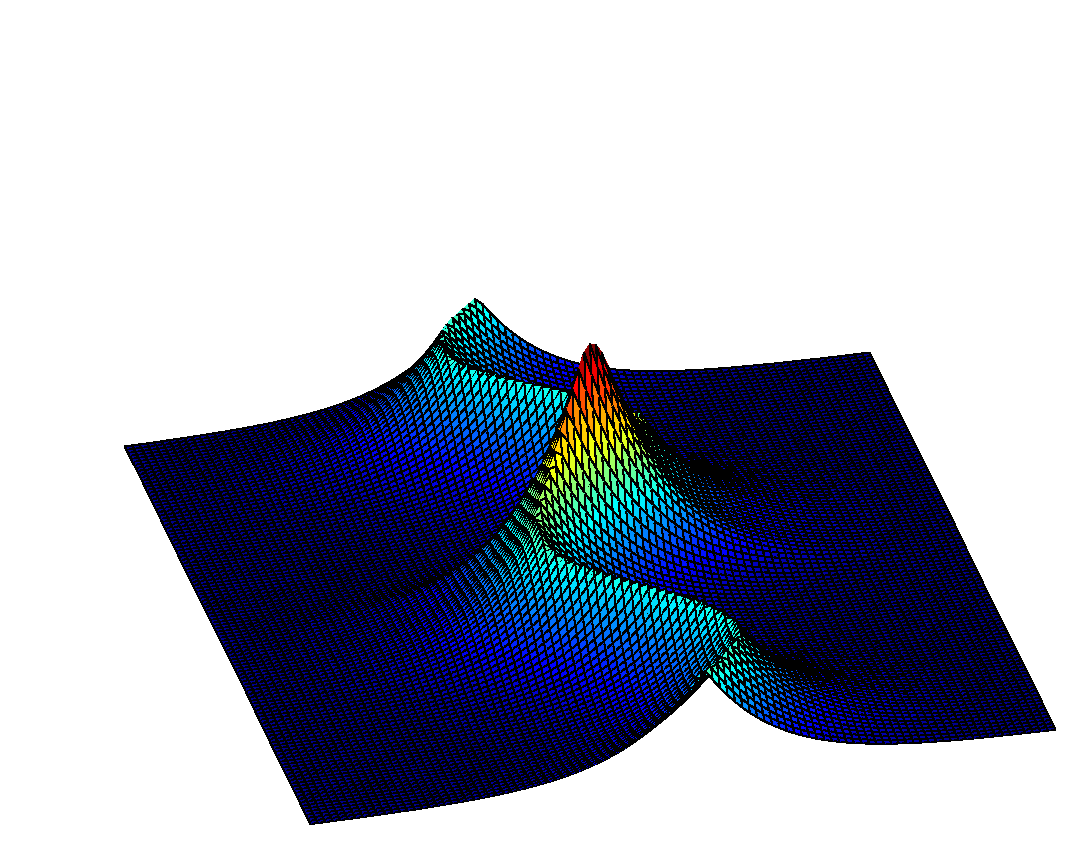
\includegraphics[scale=.80]{matlabcover}

\vskip1truein
Lance J.\ Nelson and Matthew R. Zachreson

\vskip.4truein
Department of Physics
\end{adjustwidth}

\cleardoublepage
\thispagestyle{empty}

 \begin{adjustwidth}{}{-1.5in}
 \centering
 \vspace*{1in}
 \large
 {\huge INTRODUCTION TO PYTHON}
 \vskip.4truein

 Lance J.\ Nelson and Matthew R. Zachreson
 \bigskip

 Department of Physics

 \bigskip
 Brigham Young University--Idaho

 \vfill


 {\footnotesize $\copyright$ 2017 Lance J.\ Nelson and Matthew R. Zachreson
               Brigham Young University--Idaho}

 \vskip.5truein
 {\footnotesize \emph{Last Revised: \today}}
 \normalsize

 \end{adjustwidth}

\cleardoublepage

\chapter*{Preface}

This is a tutorial to help you get started in Python. Examples of
Python code in this book are in font \code{like
this}. As you read through the text, type and execute in Python all
of the examples. Longer sections of code
are set off and named.

There are three major parts to this book: {\em Getting Started}, {\em The Basics}, and {\em Advanced Topics}.

{\em Getting Started} walks you through how to get Python installed and running, and then gives tips on what to do when your programs don't work.

We designed {\em The Basics} section to teach you Python, piece by piece.  Each chapter builds on the last, and teaches you something new. You should work through each chapter, one by one, in order.

{\em Advanced Topics} covers things that are very useful in Python, but it serves more as a reference guide.  Go through the chapters there either when you need to use what is in them, or if you just want to learn something new.  Each chapter works as a stand alone tutorial, assuming that you've already covered {\em The Basics}.

In addition to teaching you Python, this booklet can also be used as a reference manual because it is
short, it has lots of examples, and it has a table of contents and
an index.

 Please tell us about mistakes and make suggestions to improve the text
(nelsonla@byui.edu).




 \cleardoublepage \phantomsection
 \addcontentsline{toc}{chapter}{Table of Contents}
\tableofcontents

\mainmatter

\chapter{Running Python}
\label{chap:RunningPython}

\marginfig{Figures/pythonCW.jpg}{Canopy's environment for running
  Python code.}

Python is a computer programming language (don't freak out) with broad
applicability in science and engineering.  For those that are brand
new to computer programming, Python is simply a way to communicate a
set of instructions to your computer.  You'll quickly learn that your
computer is great at doing exactly what you tell it to do.  If you
find that your computer isn't doing what you think it should, it is
not because the machine is malfunctioning, rather you just probably
don't fully understand what you are telling it to do.

There are two ways to run python. One is at the command line\sidenote{If you are already comfortable with command line, then you probably don't need any help getting started. Feel free to use whatever editor you'd like. You'll need to make sure that you have Python 3 installed along with the following packages: numpy, scipy, matplotlib, ipython, sympy, and nose. These packages come pre-bundled with the Canopy distribution of Python, so if you installed Canopy, you already have them.} and the
other is through an IDE (integrated development environment). If you
don't know what the command line is, I recommend you start out using
an IDE. A good IDE for python is called Canopy, which can
be downloaded \href{https://store.enthought.com/downloads/}{here}. This text is written for Python 3, so choose the Python 3.x download that matches your operating system (Windows, Mac, or Linux).


\section{Running Your First Program}

Once you have downloaded and installed Canopy, launch the editor. You should see a window that looks similar to the one displayed in the margin. (You may have to choose "Create a new file".) The Canopy Editor has three main windows: The file browser, the editor itself, and the Python console (Labeled "Python").
The file browser shows your local file directory.  It is nice to have when you write larger Python programs. To keep big programs easy to read, we often break them into several files.
The editor itself will be where we write our Python programs. We'll address the Python Console in a moment. Right now, type

\begin{Verbatim}
print('Hello World')
\end{Verbatim}

into the editor. Save your program as \code{myFirstProgram.py}, then click the green
arrow above the editor. If you look down at the console it should say:

\begin{Verbatim}
%run "where you saved the file/myFirstProgram.py"
Hello World
\end{Verbatim}
(If you don't see the words "Hello World", double check that what you've written in the editor and matches the above code exactly.) Congratulations, you just ran your first Python program. You told the computer to write "Hello World" on the console.
Now try changing this line:
\begin{Verbatim}
print('Hello World')
\end{Verbatim}
to this:
\begin{Verbatim}
print('I can do python!')
\end{Verbatim}
and run your program again.\sidenote{You only need to do a "save as" on new files. Once you've given it a filename, Canopy will save and run your file every time you click the green arrow button.}
\section{The Python Console}
The Python console serves two purposes: First, it shows our program's outputs. (The "Hello World" from earlier.) Second, it allows us to do interactive Python. Try typing
\begin{Verbatim}
print('Hello World')
\end{Verbatim}
directly into the console, then press enter.  You should see it print
\code{Hello World}, just like it did for your program. The console
will run any Python command that you enter into it. It can be very
useful for short, quick calculations, or for looking at data when you
are trying to figure out what your program is doing. However, it is
impossible to save the commands that you enter into the console, so
you should do most of your programming in the editor.


\section{It's a Calculator}
The very easiest, yet meaningful thing you can with Python is to
perform simple math. Simple math can be performed pretty much just as
you would expect. Here are a few examples\sidenote{The \code{#} marks something called a comment.  Python knows to ignore anything on a line that comes after a \code{#}.  They exist so that you can leave notes to anyone reading the program, without affecting what the program does.}
\begin{Verbatim}
print(1+2)
print(5.0/6.0)
print(5**6)  # 5 raised to the power 6
print(678 * (3.5 + 2.8)**3.)
\end{Verbatim}
Note that typing the calculation alone, without the \code{print}
statement, will not produce any output to the screen.  Even though the
calculation has been performed, you will not see the result unless you
\code{print} it. Throughout this book, the \code{print}
statement will usually be omitted in code examples to maintain
brevity.  You should always print your result so you can see what you
have done.

\chapter{Variables and Data Types}
\label{chap:variablesDataTypes}

\marginfig{Figures/pythonCW.jpg}{Canopy's environment for running
  Python code.}


When writing a computer program, there are several big ideas, or main
pillars, that you should grasp to be successful.  Two of those pillars
are variables and functions. This chapter will focus on assigning,
manipulating, and using different variable types.  Later chapters will
focus on other main ideas and some more specific tasks that can be
accomplished using these foundational ideas.

The simplest, and most fundamental object when programming a computer
is the variable, which is nothing more than a name which is given to a
piece of information. It allows the information to be saved (stored)
so that it can be recalled and used later.  \index{Data types} There
are different types of variables and each has it's use and
limitations.  Python has many types of variables, but you will mostly
use the following types: integers, floats, lists, and arrays.  What
follows is a brief description of each variable type (we'll save our
discussion of arrays until later) with some examples to illustrate.

\section{Integer variables}
Some of you may be used to programming in C++\sidenote{C++ is a
  compiled language, whereas Python is an interpreted language}, where
the variables are declared before a value is assigned.  In python,
variables are created and assigned in one statement using the
assignment operator (\code{=}).  The simplest type of data is an
integer, a decimal-less number.  An integer variable is created and
assigned a value like this:\index{Assigning values}
\begin{Verbatim}
a = 20
\end{Verbatim}
This statement creates the variable \code{a} and assigns it a value of
$20$ (an \textbf{integer}).  The value of \code{a} can be modified in
any way you choose.  For instance, the statement
\begin{Verbatim}
a = a + 1
\end{Verbatim}
adds one to whatever value was previously stored in
\code{a}. \sidenote{An assign statement in programming is not a
  mathematical equation.  It makes perfect sense to write
  \code{a=a+1} as assign statement: it tells the computer to get the
  value of \code{a} and add 1 to it and then store the evaluated
  quantity back in the variable \code{a}.  However, the mathematical
  equation $a=a+1$ is clearly false.}  Note that {\it variable names
  in Python are case sensitive,} so watch your capitalization.
\index{Case sensitive} 
You can define multiple variables by putting the assignements on
seperate lines:
\begin{Verbatim}
a = 2
b = 4
c = a * b
\end{Verbatim}
Here we have stored the value $2$ in \code{a}, the value $4$ in
\code{b} and then used those assignments to calculate a new value: $ 2
\times 4$ and assign that value to the variable \code{c}.
%\reminder{\lefthand}{If you are using version 3 or higher of python,
%  printing a variable is done like this: \code{print(a)}.}
Other common mathematical operations can be performed on integer
variables.  For example:
\begin{Verbatim}
a = 20
b = 15
c = a + b  # add two numbers
d = a/b    # divide two numbers
r = a//b   # return only the quotient(an integer) of the division
r = a % b   # return only the remainder(an integer) of the division
e = a * b  # multiply two numbers together
f = c**4   # raise number to a power (use **, not ^)
\end{Verbatim}
Notice that performing an operation on two integers \ul{usually}
yields another integer.  The one exception is division if you are
using Python version 2 or earlier.  This can pose a serious problem if
you think about it for a second.  For example, what would be the value
of \code{d} above if the result has to be an integer?

\section{Float variables}
Most meaningful calculations should be performed using floating point
numbers, or floats in Python.  Float variables are created and assigned in
one of two ways.  The first way is to simply include a decimal place
in the number, like this
\begin{Verbatim}
a = 20.
\end{Verbatim}
You can also cast an integer variable to a float variable using the
\code{float} command
\begin{Verbatim}
a = 20
b = float(a)
\end{Verbatim}
You may wonder what would happen when a float and an integer are used
in a calculation, like this
\begin{Verbatim}
a = 0.1
b = 3 * a  #Integer multiplied by a float results in a float.
\end{Verbatim}
\marginpar{\footnotesize\captionsetup{type=table}
  \vspace{-2.5in}
\begin{tabular}{lp{1.05in}}
\texttt{abs(x)} & Find the absolute value of x\\ \\
\texttt{divmod(x,y)}        & Returns the quotient and remainder when
using long division.\\ \\
\texttt{x \% y}      & Return the remainder of $\frac{x}{y}$ \\ \\
\texttt{float(x)}      & convert \texttt{x} to a float. \\ \\
\texttt{int(x)}      & convert \texttt{x} to an integer. \\ \\
\texttt{round(x)}  & Round the number \texttt{x} using standard
rounding rules \\ \\
\end{tabular}
\captionof{table}{A sampling of built-in functions commonly used with integers
  and floats.\label{tab:HousekeepingFloats}}
}.  
The result of such a calculation is always a float.  Only when
all of the numbers used in a calculation are integers is the result an
integer.
Floats can be entered using scientific notation like this
\begin{Verbatim}
1.23e15
\end{Verbatim}

\section{Boolean variables}
A boolean variable is one that stores one of two possible values: True
or False.  A boolean variable is created and assigned similar to the
other variables you've studied so far
\begin{Verbatim}
myVar = True
\end{Verbatim}
The purpose for using a boolean variable will become more clear as you
study loops and logical statements, so stay tuned.

\section{Lists}
It is very important that you fully grasp the concept of a list
variable.  They are heavily-used in mathematical and scientific
programming.  You can think of a list as a container that holds
multiple pieces of information. The list could hold integers, floats,
strings, or really just about anything.  Let's see how we might create
a list.

\subsection*{Creating Lists}
The easiest way to create  a list is by putting the list element
inside of square brackets, like this:
\begin{Verbatim}
a = [5.6 , 2.1 , 3.4 , 2.9]
\end{Verbatim}
Note that square brackets (\code{[]}) must be used when creating the
list. If you accidentally use parenthesis (\code{()})\sidenote{Use
  parenthesis to create a tuple, which is just like a list but cannot
  be modified.}  or curly brackets (\code{\{\}})\sidenote{Use curly
  brackets to create a dictionary, which is like a list but can be
  indexed on any data type, not just integers} you'll end up creating
something other than a list.  
Another way to create a list is with
Python's \code{range} function:
\begin{Verbatim}
a = range(10,52,3)
\end{Verbatim}
This will construct a list of \ul{integers} starting at $10$, ending at
$52$, while stepping in increments of $3$. This function can also be
called with $1$ or $2$ arguments and default values will be assigned
to the missing ones.
\begin{Verbatim}
a = range(3,9)  # Creates a list starting at 3, ending a 9 stepping
                # in increments of 1 (default value)
b = range(10)   # Creates a list starting at 0(default), ending at 10 stepping
                # in increments of 1(default value)
\end{Verbatim}
\noindent You can make a list of anything.  For example, here is a
list of strings:
\begin{Verbatim}
a = ['Physics' , 'is' , 'so' , 'great']
\end{Verbatim}
The individual elements of any list need not be the same type of
data.  For instance, the following list is perfectly valid
\begin{Verbatim}
# Here is a list of strings and integers
a = ['Ben',90,'Chad',75,'Andrew',22]
\end{Verbatim}
You can even define a list of lists:
\begin{Verbatim}
a = [[4,3,2],[1,2.5,90],[4.2,2.9,10.5],[239.4,1.4],[2.27,98,234,16.2]]
\end{Verbatim}
\subsection*{Accessing and Slicing lists}
Accessing an element of a list (this will be done frequently so pay
attention!) can be accomplished using square brackets, like this
\begin{Verbatim}
a[0]  # Access the 1st element of array a
a[4]  # Access the 5th element of array a
a[-1] # Access the last element of array a
a[-2]  # Access the second to last element of array a
\end{Verbatim}
Take special note to the last two statements where a negative index is
used.  Using a negative index means that you are counting from the
back of the list forward.
Please note that python lists are zero-indexed: the first element of
any list is 0, the second element is 1, etc.  Lists can be easily
modified by specifying which element you want to change and what you
want it changed to:
\begin{Verbatim}
a = ['Physics' , 'is' , 'so' , 'great']
a[3] = 'tough'  # Change the 4th element of a to "tough"
\end{Verbatim}
At times you may want to access entire sections of list, though not
the entire list.  You can do this with the \code{:} operator, like
this
\begin{Verbatim}
aList = [4,5,10,1560,23,19]
aList[1:]
aList[1:3]
aList[:3]
aList[1:4:2]
\end{Verbatim}
There can be three numbers inside the brackets, each seperated by the
\code{:} symbol, like this \code{[x:y:z]}.  The section of the
list that is extracted starts at element \code{x}, ends at element
\code{y} (but does not include element \code{y}), while stepping in
increments of \code{z}.  Note that the last number is optional, and
omitting it will result in a default value of 1 for the step size.


When working with a list of list (also called a 2-dimensional list)
accessing an individual element requires two indices, like this
\begin{Verbatim}
a = [[4,3,2],[1,2.5,90],[4.2,2.9,10.5],[239.4,1.4],[2.27,98,234,16.2]]
c = a[3][1]
\end{Verbatim}
Here \code{[3][1]} means we are accessing the 2nd element of the 4th
list. (remember: Python lists are zero-indexed) 
 \marginpar{\footnotesize\captionsetup{type=table}
  \vspace{-4.5in}
\begin{tabular}{lp{1.05in}}
\texttt{a[x]}        & Access element \texttt{x} in list \texttt{a}\\
\texttt{a[x:y:z]}        & Extract a slice of list \texttt{a}\\
\texttt{a.append(x)}        & Append \texttt{x} to list \texttt{a} \\
\texttt{a.pop()}      & Remove the last element of list \texttt{a}. \\
\texttt{len(a)}  & Find the number of elements in \texttt{a} \\
\texttt{range(x,y,z)}  & Create a list of integers, starting at x,
ending at y, and stepping in increments of z.\\
\texttt{a.insert(x,y)}    & Insert \texttt{y} at location
\texttt{x} in list \texttt{a} \\
\texttt{a.sort()}  & Sort list \texttt{a} from least to greatest. \\
\texttt{filter(f,x)}        & Filter list \texttt{x} using the
criteria function \texttt{f}(see lambda functions).\\
\texttt{a.reverse()}  & Reverse the order of list \texttt{a}. \\
\texttt{a.index(x)}  & Find the index where element x resides. \\
\texttt{a + b}  & Join list \texttt{a} to list \texttt{b} to form one list. \\ \\
\texttt{max(a)}  & Find the largest element of \texttt{a} \\ \\
\texttt{min(a)}  & Find the smallest element of \texttt{a} \\ \\
\texttt{sum(a)}  & Returns the sum of the elements of \texttt{a} \\ \\
\end{tabular}
\captionof{table}{A sampling of ``housekeeping'' functions for lists.\label{tab:HousekeepingList}}
} 
\subsection*{Built-in Functions for Lists}
Python has many built-in functions that work on lists.  You've already
seem some of them.  Here are a few examples
\begin{Verbatim}
myList = range(5,25,2)  # Create list starting at 5, ending at 25,
                        # in increments of 2
len(myList)             # Find how many elements are in myList
myList.append(520)      # Add the number 520 to the end of myList
\end{Verbatim}
 Here, \code{range} will create a list \underline{of integers }
starting at $5$, ending at $25$ in increments of $2$.  The
\code{len} function will find the length of a list, and
\code{append} will add an element to the end of a list.  Table
\ref{tab:HousekeepingList} lists some of the more common built-in
functions/operations for lists.  Please note that this is not a
comprehensive list.  A complete list of available function can be
found in the appendix.


\subsection*{A warning: What not to do with lists}
There are several things that seem natural to do with lists but that
should not (cannot) be done.  First, it may be tempting to associate a
2-D list with a matrix and try to use the \code{:} to slice out a
submatrix.  For example, what if you defined the following 2D list
\begin{Verbatim}
from numpy import array
a = array([[1,2,3],[4,5,6],[7,8,9]])
\end{Verbatim}
and interpreted it as this matrix:
\begin{equation}
\left( \begin{tabular}{ccc}
1 & 2 & 3\\
4 & 5 & 6\\
7 & 8 & 9\\
\end{tabular}
\right)
\end{equation}
If you wanted to slice out the following 2 x 2 sub-matrix:
\begin{equation}
\left(\begin{tabular}{cc}
5 & 6 \\
8 & 8 \\
\end{tabular}
\right)
\end{equation}
and you tried to do it like this:
\begin{Verbatim}
b[1:3][1:3] 
\end{Verbatim}
you would be disappointed to find out that it did not work.  Lesson
\#1: Don't treat 2D lists as matrices.

Second, you may feel tempted to associate a list with a mathematical
vector and try to perform vector math on them. For instance, it may
seem natural to try
\begin{Verbatim}
a = [5.1 , 3.2 , 6.8 , 9.2]
b = 5 * a
\end{Verbatim}
or
\begin{Verbatim}
a = [5.1 , 3.2 , 6.8 , 9.2]
b = [2.7 , 1.9 , 3.2 , 9.9]
c = a + b
\end{Verbatim}
Can you explain the results?  So lesson \# 2 is: Doing vector or
matrix math \underline{cannot be done with a list}.  If you were
allowed to do that, what should Python do when your lists were filled
with non-numerical data, like this:
\begin{Verbatim}
a = ['Physics', 'is']
b = ['the', 'coolest', 'topic']
c = a + b
\end{Verbatim}
  This doesn't mean that the numbers \ul{stored in
  lists} can't be extracted and used in mathematical calculations,
like this
\begin{Verbatim}
a = [4.5,8,2.1,10.8,12]
c = a[0]**a[1]  # Take the first element of a and raise it to a power
                # equal to the second element of a
\end{Verbatim}
It just means that mathematical calculations involving entire arrays
of numbers (like vector and matrix math) cannot be done using the list
data type.  However, don't think for one second that Python is unable
to handle this kind of math.  Just keep reading and you'll learn how
this is done.
\section{String Variables}
\index{Strings} String variables contain a sequence of characters, and
can be created and assigned using quotes, like this
\begin{Verbatim}
s='This is a string'
\end{Verbatim}
\sidenote{You may also enclose the characters in double quotes. }
%If you need an apostrophe in your string, repeat a single quote,
%like this:
%\begin{Verbatim}
%t='Don''t worry'
%\end{Verbatim}
Some Python functions require options to be passed to them using
strings. Make sure you enclose them in quotes, as shown
above.  There are many useful function that can be used with strings.
For example, strings can be concatenated (joined) together using the
\code{+} operator:
\begin{Verbatim}
a = 'Hello'
b = ', my name is B. Nelson'
c = a + b
\end{Verbatim}
The number of characters in a string can be calculated using the
\code{len} function.
\begin{Verbatim}
a = 'Hello'
b = ', my name is B. Nelson'
c = a + b
d = len(c)
\end{Verbatim}
Individual characters inside of a string may be accessed  and sliced
in the same way that elements of a list are accessed and sliced.
\begin{Verbatim}
a = 'Hello, my name is B. Nelson'
a[18]
a[2:15]
\end{Verbatim}
\marginpar{\footnotesize\captionsetup{type=table}
  \vspace{-2.5in}
\begin{tabular}{lp{1.05in}}
\texttt{a.join(b)}  & Join all elements in list \texttt{b} while
placing string \texttt{a} between each pair of elements.\\ \\
%\texttt{str.capitalize()}  & Capitalize all characters in string
%\texttt{str} \\ \\
\texttt{a.count(b)}  & Count the number of occurrences of
string \texttt{b} in string \texttt{a}\\ \\
\texttt{a.lower()}  & Convert upper case letters to lower case \\ \\
\texttt{a[x]}  &  Access element \texttt{x} in string \texttt{a} \\ \\
\texttt{a[x:y:z]}  &  Slice a string, starting at element
\texttt{x}, ending at element \texttt{y}, with a step size of \texttt{z} \\ \\
\texttt{a + b}  &  Concatenate strings \texttt{a} and \texttt{b}.  \\ \\
\end{tabular}
\captionof{table}{A sampling of ``housekeeping'' functions for strings.\label{tab:HousekeepingStrings}}
}
 However, you'll have little luck modifying a single character in a
string unless you first convert the string to a list, like this
\begin{Verbatim}
a = 'Hello, my name is B. Nelson'
b = list(a)  # convert string a to a list
b[18] = 'S'  # Modify the 18th element in the list.
c = "".join(b)  # Join all the elements back together into one string.
\end{Verbatim}
The \code{join} function used here was probably unfamiliar to you.
It is a built-in function for use with strings.  It joins together all
of the elements in list \code{b} into one string, putting whatever
is in "" in between
each element.  There are many built-in functions that can be used with
strings.  Some of the more commonly used ones are shown in Table \ref{tab:HousekeepingStrings}
\section{Displaying Results}
It's great to calculate something useful, but not that helpful unless
you can see it.  Beginners often ask the question, ``I calculted XX
but Python didn't do anything.''  Actually, Python did exactly what
you told it:  It calculted XX and called it a day.  If you want to see
XX, you have to print it.   The fastest way to see something, as
you've already seen is using the print statement:
\begin{Verbatim}
a = 5.3
b = [5,3,2.2]
c = 'Physics is fun'
print(a)
print(b)
print(c)
\end{Verbatim}
As you can see, you can \code{print} anything and Python will dump
it to screen as it pleases.  There are times when you may want to be
more careful about the formatting of your print statments.  For
example:
\begin{Verbatim}
a = 22
b = 3.5
print("Hi, I am Joe. I am {:d} years old and my GPA is: {:5.2f}".format(a, b))
\end{Verbatim}
Notice the structure of this print statement: A string followed by the
\code{.} operator and the \code{format()} function. The variables to
be printed are provided as arguments to the \code{format} statement
and are inserted into the string sequentially wherever curly braces
(\code{\{\}}) are found.  The odd characters inside of the curly
braces are a format code: they indicate how you would like the
variable formatted when it is printed. The \code{:d} is used to
indicate an integer variable and \code{:f} is used for floats.
Further specifications regarding spacing can also be made.  The
\code{5.2} in the float formatting indicates that I'd like the number
to be displayed with at least 5 digits and 2 numbers after the
decimal.  A summary of what is available is given in table
\ref{tab:HousekeepingFormat}

\marginpar{\footnotesize\captionsetup{type=table}
  \vspace{-2.5in}
\begin{tabular}{lp{1.05in}}
\texttt{\{:4d\}}  & Display integer with 4 spaces\\ \\
\texttt{\{:.4f\}}  & Display float with 4 numbers after the decimal\\ \\
\texttt{\{:8.4f\}}  & Display float with at leasat 8 total spaces and 4 numbers after the decimal\\ \\
\end{tabular}
\captionof{table}{Formatting strings available when printing.\label{tab:HousekeepingFormat}}
}












\chapter{Functions and Libraries}
\label{chap:Functions}

One of the most fundamental constructs for any programming language is
the function. A function is nothing more than a set of instructions
packaged up and given a name.  The function can be as long and complex
or short and succinct as you wish.

The main purpose of a function is to take in information, do some calculations with or otherwise manipulate that information, then produce a result.  Here's a function you should already be comfortable with:
\begin{Verbatim}
print('Print is a function.')
\end{Verbatim}
The \code{print} function takes a string, and tells the computer to write that string to the console.

You do not need to know all of the details of how a function works in order to use it.  You just need to know what to give it, and what the result is.

All Python functions have the same general format: first you type the name of the function (\code{print}), then you put round parentheses \code{()} around whatever information\sidenote{Not all Python functions require inputs.  You use those by typing the name of the function followed by empty parentheses \code{()}.} you are giving to the function.  If a function needs more than one piece of information, you separate them with a comma:
\begin{Verbatim}
x=[1,2,3]
y=[4,5,6]
zipped=zip(x,y) #Join two lists into one, item by item
print(zipped)
\end{Verbatim}

You can think of a function as a
black box. Someone created the contents of the box, specified what
information needs to enter the box for it to be able to accomplish
its task, and what information will exit the box.  Why a black box?
Well, one benefit of functions is that the user doesn't need to
know what's inside.  They only need to know what information the box
needs and what information the box will give back to them.

Python functions generally fall into three groups: functions that come standard with Python (called native functions), functions that you can import into Python, and functions that you write yourself.

\section{Native functions}
There are a few functions that are always ready to go whenever you run Python. They are included with the
programming language.  We call these functions native
functions.  You have already been using some
of them, like these
\begin{Verbatim}
len(mylist)  # Returns the length of a list.
float(5)     # Converts an integer to a float.
str(67.3)    # Converts a float to a string.
\end{Verbatim}
The functions: \code{len}, \code{float}, and \code{str} are all
built-in functions, and they each take a single argument.  Other
useful built-in functions can be found in margin tables
\ref{tab:HousekeepingFloats}, \ref{tab:HousekeepingStrings}, \ref{tab:HousekeepingList}, and \ref{tab:HousekeepingFormat}.





\section{Imported Functions and Libraries}
Many times, you will need to go beyond what Python can do by itself\sidenote{For example, Python doesn't include \code{sin()} and \code{cos()} as Native functions.}. However, that doesn't mean you have to create everything you need to do from scratch.  Most likely, the function that you need has already been coded. Somebody
else created the function and made it available to anyone
who wants it.  Groups of functions that perform similar tasks are
typically bundled together into libraries ready to be imported so that the functions that they contain can be used.

It is critical that you know what information(variables) the function expects you to give it and what
useful information the function will give back to you.  This
information can be found in the library's documentation. Most libraries have great documentation with lists of the included functions, what the functions do, what the functions expect, and examples on how to use the most common ones.  You can usually find the library documentation by searching the internet for the library's name, plus "Python documentation".

Providing a complete list of all available libraries and function is well beyond
the scope of this book. Instead, we'll illustrate how to import
functions and use them.  As you use Python more and more you
should get in the habit of searching out the appropriate library to
accomplish the task at hand. When faced with a task to accomplish,
your first thought should be, `` I'll bet somebody has already done that.
I'm going to try to find that library.''



Let's see how to import libraries and use their functions\sidenote{Using the functions inside a libary requires that you know what
functions are available.  This information is usually available in the
library's documentation.  Google will be a great resource here.}. You've
already seen how to perform very simple mathematical calculations. ($5/6, 8^4$,
etc..)  For more complex
mathematical calculations, like $\sin(\frac{\pi}{2})$ or $e^{2.5}$,
you'll need to import these functions from a library.
\begin{Verbatim}
import math
\end{Verbatim}
This imports a library called \code{math}.  This command is like telling Python to go get the \code{math} book off of the shelf.  Functions inside the
math library can be used like this
\begin{Verbatim}
math.sqrt(5.2)  # Take the square root of 5.2
math.pi         # Get the value of pi
math.sin(34)    # Find the sine of 34 radians
\end{Verbatim}
The \code{math.} before each function is equivalent to telling Python "Use the \code{sqrt()} function that you find in the \code{math} book I told you to grab." If you just type
\begin{Verbatim}
sqrt(5.2)
\end{Verbatim}
Python won't know where to find the \code{sqrt} function and will give you an error.



A library can be imported and then called by a different name like
this:
\begin{Verbatim}
import math as mt
\end{Verbatim}
Here, the short name \code{mt} was chosen for this library.  This tells Python "I'm going to call the \code{math} book \code{mt}."
The desired functions can then be called like this
\begin{Verbatim}
mt.sqrt(5.2)  # Take the square root of 5.2
mt.pi         # Get the value of pi
mt.sin(34)    # Find the sine of 34 radians
\end{Verbatim}

Sometimes you may not want to import the entire library, just a few
functions. This can be done like this
\begin{Verbatim}
from math import sqrt,sin,pi
\end{Verbatim}
This code tells Python "Go grab \code{sqrt}, \code{sin}, and \code{pi} from the \code{math} book.  Then, you can use the \code{sqrt} and \code{sin} functions
without the library name before it, like this
\begin{Verbatim}
sqrt(5.5)
sin(pi)
\end{Verbatim}
but, you will only have access to the functions you imported, not all of the functions in the \code{math} library.

If you want to import every function inside of a library and not have to use a prefix, do this\sidenote{For larger libraries, importing all of the
  functions this way can take a long time.  A better choice is to import only
  the functions that you need.  You will also get some unexpected results if you use this method to import two different libraries that have functions with the same name.}
\begin{Verbatim}
from math import *
\end{Verbatim}
Now, every function contained in \code{math} is available without
needing the \code{math.} prefix in front of it.

\section{User-defined functions}
Sometimes, you will need to do something over and over again that you
can't find in a library.  You (the programmer) will need to write your
own function. You do it like this:
\begin{Verbatim}
def myFunction(a,b):
    c = a + b
    d = 3.0 * c
    f = 5.0 * d**4
    return f
\end{Verbatim}
This function performs several simple calculations and then uses the
\code{return} statement to pass the final result back out of the
function (the thing that exits the black box). Every user-defined function must
begin with the keyword \code{def} followed by the function name (you
can choose it). Python does not use an \code{end} statement or
anything like it to signal the end of a function.  Instead, it looks
for indentation to determine where the function ends.


The function can be called like this
\begin{Verbatim}
def myFunction(a,b):
    #Everything that is part of the function
    #needs to be indented.
    c = a + b
    d = 3.0 * c
    f = 5.0 * d**4
    return f
#The rest of this code is not part of this function.
r = 10
t = 15
result = myFunction(r,t)
\end{Verbatim}
In this case, when the function is called, \code{a} gets assigned the
value of $10$ and \code{b} gets assigned the value of $15$.  The
result of this calculation (\code{f}) is passed out of the function
and stored in the variable \code{result} for later use.


A word on local vs. global variables is in order here.  In the example
above, the variables: \code{a},\code{b},\code{c},\code{d}, and
\code{f} are \ul{local variables}.  This means that these variables
are used by the function when it is called and then immediately
forgotten.  To see what I mean try the following and observe the
results

\begin{Verbatim}
result = myFunction(r,t)
print(c)
\end{Verbatim}
Notice the error since Python does not remember that inside the function \code{c=a+b}.

In contrast, the variables \code{r},\code{t}, and \code{result} are
called \ul{global variables}, which means that Python remembers these
assignments from anywhere, including inside of functions.  So,
technically, you could do the following:

\begin{Verbatim}
g = 9.8         #<--- g defined to be a global variable
def myFunction(a,b):
    c = a + g   # <--- Notice the reference to ``g'' here
    d = 3.0 * c
    f = 5.0 * d**4
    return f
#The rest of this code is not part of this function.
r = 10
t = 15
result = myFunction(r,t)
\end{Verbatim}
and there would be no error.  Notice that \code{g} has been defined as
a \ul{global variable}, and the function \code{myFunction} knows it's
value and can use it in a calculation.  \textbf{\ul{ Using global
    variables is usually considered to be bad form and confusing.}}
If you are going to use global variables there better be a very good
reason.  For example, assigning physical constant, like $k_B$, $G$, or
$\epsilon_0$, to be global variables is one example of proper use
because their values never change and may be used repeatedly in
multiple functions.  Generally speaking however, every variable that
is used in a function ought to be either i) passed in, or ii) defined
inside of the function.

Let's look at one more example.  Here's (roughly) what Python does
every time you use \code{math.sin(x)}:
\begin{Verbatim}
def sin(x):
    from math import factorial
    result=0
    for k in range(20): #This Starts a "for loop"
        sign=(-1)**k
        denom=factorial(2*k+1)
        result+=sign*x**(2*k+1)/denom
    return result
\end{Verbatim}
This function takes in a number (\code{x}) and returns the sine of \code{x}.  When you use \code{sin()}, the rest of your program has no idea that the variables \code{result}, \code{k}, \code{sign}, and \code{denom} were assigned along the way.  The main program only knows that \code{sin()} took \code{x} and returned a number that has the value of $\sin(x)$.

\subsection*{Importing User Defined Functions}
If you ever write a function that you find yourself using over and over again, or if you've written so many functions for a program that it makes your program hard to read, you can save your functions in another file and import them just like a Python library.

As an example, assume that you've written your own \code{sin}, \code{cos}, and \code{sum} functions and saved them in a file called \code{my_funcs.py}.  As long as the program that will use these functions is saved in the same folder\sidenote{You can specify a path to a different folder during your import, or make your functions available to any program using Python on your computer.  However, the steps to do so are beyond the scope of this book.}, you can import and use them like any other library.
\begin{Verbatim}
#Method #1
import my_funcs
my_funcs.sin(15)

#Method #2
from my_funcs import sin
sin(15)

#Method #3
import my_funcs as mf
mf.cos(50)

#Method #4
from my_funcs import *
cos(50)
\end{Verbatim}




\chapter{Calculating}
\label{chap:Calculating}
In a scientific setting, much of what you will ask Python to do will
involve math.  You've already seen how to do very simple math. Here we
will give you all the tools you will need to do any mathematical
calculation you could want.

The calculations that you will perform can be roughly categorized into
two types: (i) simple calculations involving a couple of numbers ( e.g.
$5.5 \sin(6.2 \times \frac{\pi}{2})$ or $5.5 J_0(3.5 \times
\frac{\pi}{4})$) and (ii) more complicated calculations involving many
numbers (e.g. $5.5 \sum_i (x_i - D)^2$ where $x$ is a list of 200,000
numbers)
\section{Simple Calculations}
Any mathematical function that you could possibly need to perform a
simple calculation can be found in the library \code{numpy} or
\code{scipy}. Here is an example:
\begin{Verbatim}
from numpy import sin, pi
from scipy.special import j0 # Bessel function of the 1st kind of
                             # order 0

a = 5.5
b = 6.2
c = pi/2
d = a * sin(b * c)
e = a * j0(3.5 * pi/4)
\end{Verbatim}

Most likely, \code{Numpy} has the mathematical function that you need
and if it doesn't, then \code{scipy.special} probably has it. Tables
\ref{tab:Numpy} and \ref{tab:Scipy} provide a small sampling of the
functions available.  See online help for a more extensive listing.

\section{More Complex Calculations: Don't Use Lists}
What about more complicated calculations involving large data sets?
It may {\em seem} natural to use a list to perform this type of calculation.
However, lists were not designed to do math. For example,
suppose you defined the following list:
\begin{Verbatim}
a = [5.1 , 3.2 , 6.8]
\end{Verbatim}
conceptualizing it as a mathematical vector, and then tried to calculate:
\begin{Verbatim}
b = 3 * a
\end{Verbatim}
expecting \code{b} to become \code{[15.3,9.6,20.4]}.  Try it.  Can you
explain the result? Or maybe you define two lists and try to add them
up, like this:
\begin{Verbatim}
a = [5.1 , 3.2 , 6.8 , 9.2]
b = [2.7 , 1.9 , 3.2 , 9.9]
c = a + b
\end{Verbatim}
Can you explain the results?  So lesson \# 1 is: \ul{Lists} are not
mathematical vectors or matrices and doing vector or matrix math
\underline{cannot be done with a list}.  If you were allowed to do
that, what should Python do when your lists were filled with
non-numerical data, like this:
\begin{Verbatim}
a = ['Physics', 'is']
b = ['the', 'coolest', 'topic']
c = a + b
\end{Verbatim}
  This doesn't mean that the numbers \ul{stored in
  lists} can't be extracted and used in mathematical calculations,
like this
\begin{Verbatim}
a = [4.5,8,2.1,10.8,12]
c = a[0]**a[1]  # Take the first element of a and raise it to a power
                # equal to the second element of a
\end{Verbatim}
it just means that mathematical calculations involving entire arrays
of numbers cannot be done using the list data type.

Second, it may be tempting to associate a
2-D list with a matrix and try to use the \code{:} to slice out a
submatrix.  For example, what if you defined the following 2D list
\begin{Verbatim}
from numpy import array
a = [[1,2,3],[4,5,6],[7,8,9]]
\end{Verbatim}
and interpreted it as this matrix:
\begin{equation}
\left( \begin{tabular}{ccc}
1 & 2 & 3\\
4 & 5 & 6\\
7 & 8 & 9\\
\end{tabular}
\right)
\end{equation}
If you wanted to slice out the following 2 x 2 sub-matrix:
\begin{equation}
\left(\begin{tabular}{cc}
5 & 6 \\
8 & 9 \\
\end{tabular}
\right)
\end{equation}
and you tried to do it like this:
\begin{Verbatim}
a[1:3][1:3]
\end{Verbatim}
you would be disappointed to find out that it did not work that way.
You should take a few minutes to understand what it did do.  In the
end you should always remember to \ul{not treat 2D lists as matrices}.

However, don't think for one second that Python is unable
to handle this kind of math.  Just keep reading and you'll learn how
this is done using the Numpy library. (pronounced num-pie, short for numerical
Python)


\section{Numpy Arrays}
If lists are not designed for mathematical calculations, what should
be used to do this sort of thing.  The answer is a Numpy array. Let's
explore this a little more carefully using a specific example that is
designed to help you see what we mean.  Let's say
you have a large data set
\begin{Verbatim}
x = [2.42762254  2.53691271  3.15932278  1.7128872   2.54105921  2.54094893
  2.55284336  2.36430906  2.37972415  2.70342833  2.2846214   2.37636944
  2.74236195  3.06429336  2.29889954  1.99944808  2.46066766  1.86346638
  2.69619554  1.81298331  2.96144256  3.020208    2.71914935  2.59783385
  2.41512769  2.84674515  2.92394769  3.15879826  2.25886137  3.04074924
  3.14635756  2.60488105  2.79643916  2.67695452  2.77874282  1.94903284
  2.60399377  1.88255081  2.38624122  3.43726289  2.46514806  2.74985076
  2.33684695  2.58710514  2.10996793  3.19191947  3.93418676  2.90987071
  2.52449511  1.71514896  2.42465365  2.24485334  2.88390193  2.97911184
  2.86770773  2.97543667  2.00454583  2.56522443  2.99691011  2.79259592
  2.01617544  1.66098216  2.59230004  2.31295971  3.49570792  2.37890997
  2.14965171  2.40578128  2.44831872  2.0519382   2.41011389  3.07252157
  2.50662296  2.49878442  1.97225157  2.00764702  2.67472532  3.02465629
  2.45257132  2.9325564   2.69301075  2.81356219  2.49886432  1.97998459
  2.86166356  3.24091275  2.83846089  2.58103089  2.23525104  2.85815534
  3.33391592  2.6850452   2.3267767   3.27800198  2.17433118  2.17612604
  2.80002452  2.48975877  3.01856681  2.34280246]
\end{Verbatim}
and you want to calculate the summation
\begin{equation}\label{eq:sum}
\sum_{i=1}^N (x_i - D)^3
\end{equation}
where $x_i$ are the data given above and $D = 5$.  You could
calculate, one-by-one, each contribution in the sum and then add them
up.  However, there is an easier way involving
a library called \code{numpy} .  The main object used in this library
is called an \code{array}, which is very similar to a list except that
an array is intended for mathematical use.  If \code{x} were a Numpy
array, the code to evaluate the sum in equation \ref{eq:sum} would be
as simple as:
\begin{Verbatim}
D=5 #define D so the next line looks exactly like the equation
my_sum=sum((x-D)**3)
\end{Verbatim}

Let's explore arrays a little more.

\subsection*{Array Creation}
There are several ways to create an array.  If you already have a list
of numbers and you just want to convert it to an array, you can do it
with \code{numpy}'s \code{array} function:
\begin{Verbatim}
from numpy import array
xList = [2 , 3 , 5.2 , 2 , 6.7]
xArray = array(xList)
\end{Verbatim}
If you are looking for a function to create an array from scratch,
there are plenty of options.  The function \code{arange} is very similar to
the native \code{range} function that you have already seen.  The
difference is that \code{arange} creates an array object instead of
a list object and \code{arange} allows the stepsize to be less than
one.  Here is an example:
\begin{Verbatim}
from numpy import arange
myArray = arange(0,10,.1)
\end{Verbatim}
This will create an array that looks like this:
\begin{Verbatim}
[0,.1,.2,.3,.4,.5,.6.... 9.5,9.6,9.7,9.8,9.9]
\end{Verbatim}
\marginpar{\footnotesize\captionsetup{type=table} \vspace{-1.5in}
\begin{tabular}{lp{1.05in}}
\code{logspace}        & Returns numbers evenly spaced on a
log scale.  Same arguments as \texttt{linspace}\\ \\
\code{empty}        & Returns an empty array with the
specified shape\\ \\
\code{zeros}        & Returns an array of zeros with the
specified shape\\ \\
\code{ones}        & Returns an array of ones with the
specified shape.\\ \\
\code{zeros\_like}        & Returns an array of zeros with the
same shape as the provided array. \\ \\
\code{fromfile}        & Read in a file and create an array from the
data.\\ \\
\code{copy}        & Make a copy of another array.\\ \\
\code{mgrid}        & Create coordinate matrices from coordinate vectors.\\ \\
\code{meshgrid}        & Create coordinate matrices from coordinate vectors.\\ \\
\end{tabular}
\captionof{table}{A sampling of array-building functions in
  numpy. The arguments to the functions has been omitted to maintain
  brevity.  See online documentation for further details.\label{tab:Arraybuilding}}
}
 Another very useful function for array-creation is \code{linspace},
which creates an array by specifying the starting value, ending value,
and the number of elements that the array should contain.  For example:
\begin{Verbatim}
from numpy import linspace
myArray = linspace(0,10,10)
\end{Verbatim}
This will create an array that looks like this:
\begin{Verbatim}
[0,1.11111,2.222222,3.333333,4.4444444,5.55555555,6.666666,
            7.7777777,8.8888888,10]
\end{Verbatim}
When you use the \code{linspace} function, you aren't specifying a
step size: the distance between values in the array.  You can ask the
\code{linspace} command to tell you what step size results from the
array that it created by adding the \code{retstep =True} as an
argument to the function,like this:
\begin{Verbatim}
from numpy import linspace
myArray,mydx = linspace(0,10,10,retstep = True)
\end{Verbatim}
Notice that since \code{linspace} is now returning two things(the
array and the step size), we must have two variables to assign them to
on the left hand side of the equals sign.

Many other useful function for creating arrays are available.  Online
documentation is freely available.  Table \ref{tab:Arraybuilding}
gives some of the more heavily-used ones:

\subsection*{Simple Math with Arrays}
Once the array object is created, a whole host of mathematical
operations become available.  For example, you can square the array
and Python knows that you want to square each element, or you can add
two arrays together and Python knows that you want to add the
individual elements of the arrays.  You can add a constant value to
every element of an array, or even multiply two arrays together and
the elements of the first array are multiplied by the corresponding
element in the second.  Here's a sampling of examples.
\begin{Verbatim}
from numpy import array
xList = [2 , 3 , 5.2 , 2 , 6.7]
xArray = array(xList)    # Create first array
yArray = array([4,8,9.8,2.1,8.2,4.5])  # Create second array

c = xArray**2   # Square the elements of the first array
d = xArray + 3  # Add 3 to every element of the first array
e = xArray * 5  # Multipy every element of the first array by 5
f = xArray + yArray  # Add the elements of array one to the elements of
                     # array two
g = xArray * yArray  # Multiply the elements of array one by
                     # the elements of array two

\end{Verbatim}
In short, you can do all of the math that you were hoping you could do
when you first learned about Python lists.

\subsection*{Mathematical functions with Arrays}
\marginpar{\footnotesize\captionsetup{type=table}
  \vspace{0.5in}
\begin{tabular}{l}
\texttt{sin(x)} \\
\texttt{cos(x)} \\
\texttt{tan(x)} \\
\texttt{arcsin(x)} \\
\texttt{arccos(x)} \\
\texttt{arctan(x)} \\
\texttt{sinh(x)} \\
\texttt{cosh(x)} \\
\texttt{tanh(x)} \\
\texttt{sign(x)} \\
\texttt{exp(x)} \\
\texttt{sqrt(x)} \\
\texttt{log(x)} \\
\texttt{log10(x)} \\
\texttt{log2(x)} \\
\end{tabular}
\captionof{table}{A very small sampling of functions belonging to the
  \texttt{numpy} library.\label{tab:Numpy}}
}

Mathematical functions (like $\sin(x)$, $\sinh(x)$...etc.) can be
evaluated using arrays as their arguments and the result is an array
of function values.  (Just imagine wanting to calculate the $\sin$ of
1,000,000 numbers!!) However, you must use functions from either the
\code{numpy} or \code{scipy} library, and not from the \code{math}
library.  The functions from \code{numpy} and \code{scipy} library are
designed to work on arrays but the one from the \code{math} library is
not. Here is an example
\begin{Verbatim}
import numpy as np
import math

xList = [2 , 3 , 5.2 , 2 , 6.7]
xArray = array(xList)

c = np.sin(xArray)   # Works just fine, returning array of numbers.
d = math.sin(xArray) # Returns an error.
\end{Verbatim}
Notice that \code{math}'s version of \code{sin} does not
know what to do when you give it an array of numbers.  It only works
for single numbers.  \code{Numpy}'s \code{sin} function, on the
other hand, does know what to do with an array of numbers: it
calculates the sin of all the numbers.


\section{Accessing and Slicing Arrays}
Accessing and slicing arrays can be done in exactly the same way as is
done with lists.  However, there is some additional functionality for
accessing and slicing arrays that do not apply to lists.
\subsection*{Accessing Multiple Elements}
Let's consider the following 1-d array:
\begin{Verbatim}
from numpy import array
a = array([1,2,3,4,5,6,7,8,9,10])
\end{Verbatim}
Let's say you wanted to extract elements 2,3,5,and 9.  You can extract
all of these elements in one shot by using a list of these numbers for
the index, like this:
\begin{Verbatim}
b = a[[2,3,5,9]]
\end{Verbatim}
You can't do that with lists.

When using two-dimensional arrays, like this one:
\begin{Verbatim}
from numpy import array
a = array([[1,2,3],[4,5,6],[7,8,9]])
\end{Verbatim}
single elements of this array can easily be extracted, just as with
lists:
\begin{Verbatim}
from numpy import array
a = array([[1,2,3],[4,5,6],[7,8,9]])
b = a[0][2]
\end{Verbatim}
This will extract the number 3, which is the third element in the
first list.  In other words, it's element 0,2 in array \code{a}.
What if you wanted to extract multiple elements in one shot.  Could
you do that?  In fact you can and here is how:
\begin{Verbatim}
from numpy import array
a = array([[1,2,3],[4,5,6],[7,8,9]])
b = a[[0,2,1],[1,1,2]]
\end{Verbatim}
Pay special attention to the last line.  It will extract the numbers
2,8, and 6.  The first list (\texttt{[0,2,1]}) indicate the rows
(first dimension of the array) where the element is to be extracted
and the second list (\texttt{[1,1,2]}) indicate the columns that
correspond to the rows provided.  So elements \texttt{[0,1]},
\texttt{[2,1]}, and \texttt{[1,2]} from list \texttt{a} will be
extracted.  The lists of indices can be as long as you want them to be
and all of the corresponding elements will be extracted.
\subsection*{Boolean Slicing}
Imagine wanting to extract the elements of an array that meet some
provided criteria.  An array can be sliced according to the provided
criteria very easily by replacing the index with the selection
criteria as a boolean statement.
\begin{Verbatim}
from numpy import array
a = array([1,2,3,4,5,6])
b = a[a>2]
\end{Verbatim}
Here, only those elements that are greater than 2 will be extracted
from the array.  It will work on multi-dimensional arrays as well

\subsection*{Multi-dimensional Slicing}
We've already shown you how to slice a list using the \code{:}
operator.  The same can be done with arrays.  However, for 2D (and
higher) arrays the slicing is more powerful (intuitive).  It can be
helpful to visualize an array as a matrix, even if it is not being
treated that way Mathematically.  For example, let's say that you
define the following array:
\begin{Verbatim}
from numpy import array
a = array([[1,2,3],[4,5,6],[7,8,9]])
\end{Verbatim}
which could be interpreted as this matrix:
\begin{equation}
\left( \begin{tabular}{ccc}
1 & 2 & 3\\
4 & 5 & 6\\
7 & 8 & 9\\
\end{tabular}
\right)
\end{equation}
If you wanted to slice out the following 2 x 2 sub-matrix:
\begin{equation}
\left(\begin{tabular}{cc}
5 & 6 \\
8 & 8 \\
\end{tabular}
\right)
\end{equation}
you could do it like this:
\begin{Verbatim}
b[1:3,1:3]  # Slice out a sub-array (Exactly what you wanted!)
\end{Verbatim}
If you want all of the elements in a given dimension, use the \code{:}
alone with no numbers surrounding it. For example, the following:
\begin{Verbatim}
b[:,1:3]
\end{Verbatim}
would extract all of the rows on columns 1 and 2:
\begin{equation}
\left(\begin{tabular}{cc}
2 & 3 \\
5 & 6 \\
8 & 8 \\
\end{tabular}
\right)
\end{equation}
\marginpar{\footnotesize\captionsetup{type=table}
  \vspace{-1.0in}
\begin{tabular}{lp{1.00in}}
\texttt{airy(z)}& Airy function  \\
\texttt{jv(z)} & Bessel function of 1st kind\\
\texttt{yv(z)} & Bessel function of 2nd kind\\
\texttt{kv(n,z)} & Modified Bessel function of 2nd kind of integer
order n\\
\texttt{iv(v,z)} & Modified Bessel function of 1st kind of real
order v\\
\texttt{hankel1(v,z)} & Hankel function of 1st kind of real
order v\\
\texttt{hankel2(v,z)} & Hankel function of 2nd kind of real
order v\\
\end{tabular}
\captionof{table}{A very small sampling of functions belonging to the
  \texttt{scipy.special} library.\label{tab:Scipy}}
}
This kind of slicing just can't be done with lists.  Also note that
you must use the \code{[x1:y1,x2:y2]} notation rather than the
\code{[x1:y1][x2:y2]} notation, familiar with lists.  Use of the
latter will not fail, but it will not produce the sub-matrix desired.


\section{Miscellaneous Mathematical Functions}

\subsection*{Summing the elements}
Suppose you have a list(or array) of numbers and you'd like to add up
all of the elements.  Python has a built-in \code{sum} function and
there is also a \code{sum} function inside of \code{numpy} that
will do this. They both do the same thing for one-dimensional lists.
\begin{Verbatim}
a = [1.5,2.2,9.8,4.6]
b = sum(a)   #Use built-in sum function
from numpy import sum
c = sum(a)   # Use numpy's sum function
\end{Verbatim}
If you are summing up the elements of a two-dimensional list, the
built-in version of \code{sum} will not work and you will have to
use \code{numpy}'s version.
\begin{Verbatim}
a = [[1.5,2.2],[9.8,4.6]]  # Define a 2-d list, a list of lists
b = sum(a)   #Use built-in sum function, notice the error
from numpy import sum
c = sum(a)   # Use numpy's sum function, no error.
d = sum(a,axis = 1)
\end{Verbatim}
Notice the extra argument to the \code{sum} function in the last
line.  The \code{axis=1}\sidenote{By default, \code{axis=0}.  Therefore \code{sum(a)} and \code{sum(a,axis=0)} perform the same operation.} indicates that you want to sum up the
elements in each individual list and return a list of sums.  If you
had a higher-dimensional list, you could use \code{axis=2} or
\code{axis = 3} as well.


\marginpar{\footnotesize\captionsetup{type=table} \vspace{0in}
\begin{tabular}{lp{1.05in}}
\code{sum}& sum up the elements of an array.\\
\code{prod}& find the product of the elements of an array.\\
\code{cumsum}& cumulative sum up the elements of an array.\\
\code{cumprod}& cumulative product up the elements of an array.\\
\code{diff}        & discrete difference between all adjacent elements.\\
\code{cross}        & cross product of two vectors.\\
\code{inner}        & dot(inner) product of two vectors.\\

\end{tabular}
\captionof{table}{A sampling of miscellaneous functions in
  numpy.  See online documentation for further details.\label{tab:NumpyMisc}}
}
\section{Complex Arithmetic}
Python can work with complex numbers just as easily as real numbers.
The variable \texttt{j} is the imaginary number $\sqrt{-1}$ and a
complex number can be specified by placing the \texttt{j} after the
imaginary number:
\begin{Verbatim}
a = 1 + 2j
b = 2 + 3j
print(a+b)
\end{Verbatim}
You may also create a complex number using the \texttt{complex}
function:
\begin{Verbatim}
a = complex(1,2j)
b = complex(2,3j)
print(a+b)
\end{Verbatim}
There are several native functions that work on complex numbers:
\begin{Verbatim}
a = 1 + 2j
b = 2 + 3j
c = a.real
d = a.imag
e = a.conjugate()
\end{Verbatim}
More functions are available in the \texttt{cmath} package.

\chapter{Debugging Basics}
\label{chap:debug}
In programming, we refer to any mistakes in your code as a "bug". The term "bug" also refers to anytime your code does something that you don't expect it to.  As a programmer, you will be spending a good amount of your time trying to find and fix these bugs.  We call that "debugging".

All programmers make mistakes, even the experts.  Making bugs is such a common occurrence that it's often said, "the only bug free code is no code at all."

This chapter gives you some tips and tricks on finding your bugs.  Bugs generally come in two types: ones that break your code and ones that don't do what you think.


\section{Bugs That Break Your Code}
As Python reads through your program, if it reaches a line of code that it can't read, or doesn't know what to do with, it will stop and print out an error message.  The message that it prints out is intended to help you, so you should learn to read it.

Here's an example of an error message:
\begin{Verbatim}
Traceback (most recent call last):
  File "errorExample.py", line 136, in <module>
    calculated_var=my_func(x,y)
  File "errorExample.py", line 63, in my_func
    divisor=int(xx/y)
NameError: name 'xx' is not defined
\end{Verbatim}
Let's break it down, piece by piece, starting with:
\begin{Verbatim}
Traceback (most recent call last):
\end{Verbatim}
This lines tells you that Python is going show you the steps that led up to the error, or trace back to it.  The next several lines show you those steps.  Here's the first place Python noticed the problem:
\begin{Verbatim}
  File "errorExample.py", line 136, in <module>
    calculated_var=my_func(x,y)
\end{Verbatim}
This tells me that in my file \code{errorExample.py}, something went wrong when Python tried to execute the command \code{calculated_var=my_func(x,y)}.  The next set of lines tells me that the problem is in the function \code{my_func}:
\begin{Verbatim}
  File "errorExample.py", line 63, in my_func
    divisor=int(xx/y)
\end{Verbatim}
Specifically, something went wrong on line 63, in the file \code{errorExample.py}. Line 63 contains the code \code{divisor=int(xx/y)}.

The last line of the error statement tells me what I did wrong:
\begin{Verbatim}
NameError: name 'xx' is not defined
\end{Verbatim}
I used a variable \code{xx} without defining it first. The \code{NameError:} at the beginning tells me what kind of mistake I made, then the \code{name 'xx' is not defined} gives more details about the problem.  Here are the different types of errors that you can get, along with ideas on things you should try to fix them.

\subsection*{AttributeError}
Attribute errors occur when you try to use a method (one of the \code{.} functions) that doesn't exist.  For example,  if you set \code{x=5}, then \code{x.append(7)} will create an attribute error, since you can't \code{append} to an integer.

You will also get this error if you misspell the method.  Even if \code{y} is a list, \code{y.appned(5)} will create an error because \code{appned} isn't a method.  \code{y.append(5)} will work just fine.

\subsection*{SyntaxError}
Syntax errors occur when you've made a mistake formatting your code.  Check these sorts of things:
\begin{itemize}
\item You've forgotten a \code{:} at the end of a \code{def}/\code{if}\code{for}\code{while} line.
\item You've forgotten to put quotes around a string, or you've mismatched the type of quotes.
\item You have mismatched brackets or parentheses.
\end{itemize}
The parenthesis can be a little harder to track down, because Python will tell you the line number where it noticed there was a problem with parentheses.  Since Python also uses parentheses to break one long line of code into multiple lines, the mismatch might be earlier in your program.

\subsection*{NameError}
Name errors occur whenever Python doesn't recognize the name of a variable or a function.  Here are some common reasons:
\begin{itemize}
\item You misspelled the variable/function/method namem
\item You use a function from a package that you forgot to import
\item You forgot to define a variable
\item You use a function before you define it
\item You forgot to put quotes around a string so Python is trying to read it as a variable.
\end{itemize}

\subsection*{TypeError}
Type errors occur whenever you try to do an opperation on the wrong data type.  You can't do float operations on a list, for example.  Nor can you divide by a string.

Here's an example of the most common type error I see from beginning programmers:
\begin{Verbatim}
v=[5.0, 6.0, 7.5]
t=5.0
x=v*t
\end{Verbatim}
Python does not know how to multiply a list (\code{v}) by a float (\code{t}), so (\code{v*t}) gives a type error.

However, this code will run fine:
\begin{Verbatim}
v=[5.0, 6.0, 7.5]
t=5.0
x=v[1]*t
\end{Verbatim}
since \code{v[1]} is \code{6.0} (a float), Python has no problem multiplying \code{5.0*6.0}.

\subsection*{IndentationError}
Python uses indentation to figure out when functions and loops begin and end.  If you have too many spaces, (or too few) you will get an indentation error.

You also aren't allowed to mix tabs and spaces.  Even if two rows look like they are lined up, if one was indented with a tab and the other with a few spaces, you will get an indentation error.  If you are using Canopy, you probably won't run into this problem. Every time you use tab to indent, Canopy automatically replaces tab with four spaces.

There are a few other types of errors that you may run into, but these are the most common.  If you are ever completely stumped by an error message, you can usually find answers by just copying the error type and details (the stuff after the \code{:}) and searching for it on Google.

\subsection*{Errors When Using Imported Packages}
If you've imported a package like Numpy, and give the wrong thing to one of the Numpy functions, you will get a very long error message that lists every function that the Numpy function you used depends on.  Here's an example:

\begin{Verbatim}
Traceback (most recent call last):
  File "errorExample.py", line 4, in <module>
    plt.plot(data,y)
  File "/Users/test_usr/canopy/lib/python3.4/site-packages/matplotlib/pyplot.py", line 3099, in plot
    ret = ax.plot(*args, **kwargs)
  File "/Users/test_usr/canopy/lib/python3.4/site-packages/matplotlib/axes/_axes.py", line 1373, in plot
    for line in self._get_lines(*args, **kwargs):
  File "/Users/test_usr/canopy/lib/python3.4/site-packages/matplotlib/axes/_base.py", line 304, in _grab_next_args
    for seg in self._plot_args(remaining, kwargs):
  File "/Users/test_usr/canopy/lib/python3.4/site-packages/matplotlib/axes/_base.py", line 282, in _plot_args
    x, y = self._xy_from_xy(x, y)
  File "/Users/test_usr/canopy/lib/python3.4/site-packages/matplotlib/axes/_base.py", line 223, in _xy_from_xy
    raise ValueError("x and y must have same first dimension")
ValueError: x and y must have same first dimension
\end{Verbatim}

When that happens, the most useful thing to do is start at the top of the traceback and find the last time that it says the error is in your program.  Then, read the error at the bottom.  Here are the relevant bits of that long error message:

\begin{Verbatim}
Traceback (most recent call last):
  File "errorExample.py", line 4, in <module>
    plt.plot(data,y)
ValueError: x and y must have same first dimension
\end{Verbatim}
This lets me know that there is something wrong with my plot command on line 4. The \code{must have the same first dimension} part of the error lets me know that there is something wrong with the sizes of \code{data} and \code{y}.

\section{Bugs that don't make errors}
As you practice programming in Python, you will start to make fewer and fewer mistakes that Python will catch.  Your program will run without any errors, but it doesn't do what you expect it to.

When that happens, it tells you that you've written your Python perfectly, but you've told your computer to do the wrong thing.  For example, a plot might not have the right axes or
you might calculate a distance that is three times further than what you expected.

To catch these sorts of bugs, hunt for them with a bottom-up approach\sidenote{If you have a very large program with lots of pieces, sometimes it can be faster to do a top-down approach to find out which piece is broken, then do a bottom-up approach on just that piece.}.  Start at place furthest down in your code where you know something has gone wrong.  If you are having a problem with a plot, first check the plot commands themselves to see if everything is in order.

If everything looks ok in your plot command, check the variables that you are plotting.  If you have a problem with the command
\begin{Verbatim}
plt.plot(x,y)
\end{Verbatim}

Tell your program to print \code{x} and \code{y} just before you try to plot them:
\begin{Verbatim}
print(x)
print(y)
plt.plot(x,y)

\end{Verbatim}
then run your program again. When they print\sidenote{You can also see what is stored in the variable \code{x} by typing \code{x} into the console and hitting enter.}, check and see if \code{x} and \code{y} have the sort of information in them that you expect.  If they don't, look back at the part of the program where you made \code{x} and \code{y}, then continue looking backwards until you find your mistake.

\section{Toy Problems}
Often times when we write programs that do calculations for us, we test them out with toy problems.  For example, if you write a program that fits a line to some data, you can test it out by giving it data where you already know the slope and intercept.  If you set
\begin{Verbatim}
x=[0,1,2,3,4,5]
y=[0,1,2,3,4,5]
\end{Verbatim}
Your line fitting function should return a slope of \code{1.0} and an intercept of \code{0.0}. If it doesn't, you definitely know that you've done something wrong.

As another example, if you are writing a program that will calculate the path a projectile will take when fired through the air while including air resistance, first leave out air resistance and see if your program will match what you expect from kinematics.

Toy problems won't help you catch all of your bugs, but they are a quick and easy way to catch many of them.


\input{chapters/loopslogic}
\chapter{Basic Plotting}
\label{chap:Plotting}

Creating plots is an important task in science and engineering.  The
old addage ``A picture is worth a thousand words!'' is wrong.... it's
worth way more than that if you do it right.
\medskip

\section{Linear Plots}

\subsection*{Making a Grid}
\index{Plotting, xy} Simple plots of $x$ vs. $y$ are done using a
library called \code{matplotlib}.  In order to build make a plot, \code{matplotlib} needs arrays of $x$ and $y$ points that are going to be plotted.  It cannot generate these points on its own.
To build an array \code{x} of $x$-values
starting at $x=0$, ending at $x=10$, and having a step size of
$.01$, you'll need numpy's \code{arange} function:
\begin{Verbatim}
from numpy import arange
x=arange(0,10,0.01)
\end{Verbatim}
To make a corresponding array of $y$ values according to the
function $y(x)=\sin(5x)$ simply type this
\begin{Verbatim}
from numpy import sin
y=sin(5*x)
\end{Verbatim}
\reminder{\lefthand}{Remember that you must use \ul{numpy's} \code{sin}
  function if you want to be able to pass an array of values to it.
  Using math's version will produce an error.}
Both of these arrays are the same length, as you can check with the
\code{len} command
\begin{Verbatim}
len(x)
len(y)
\end{Verbatim}

\subsection*{Plotting the Function}
Once you have two arrays of the same size, you plot \code{y} vs.
\code{x} like this
\begin{Verbatim}
from matplotlib import pyplot
pyplot.figure()
pyplot.plot(x,y)
pyplot.show()
\end{Verbatim}
This will create a plot where the points are connected.  If you omit
the \code{pyplot.show()} command, the plot will not appear on your
screen.  You can save the plot to a file by replacing the
\code{pyplot.show()}  command with\sidenote{You determine the filetype by the file extension. \code{'filename.png'} makes a png image, while \code{'filename.pdf'} makes a pdf.}
\begin{Verbatim}
pyplot.savefig('filename.png')
\end{Verbatim}
If you want to see the actual data points being plotted, you
can either add the string \code{'ro'} inside of the plot command (the \code{'r'}
means make the data points red and the \code{'o'} means plot circle markers) or use the
\code{scatter} function, like this:
\begin{Verbatim}
from matplotlib import pyplot
pyplot.scatter(x,y)
\end{Verbatim}

\index{Array, first or second half} And what if you want to plot part
of the \code{x} and \code{y} arrays? The \code{colon} operator can
help.  Try the following code to plot the first and second half
separately:
\begin{Verbatim}
from matplotlib import pyplot
nhalf = len(x)/2
pyplot.plot(x[0:nhalf],y[0:nhalf])
pyplot.plot(x[nhalf:],y[nhalf:])
pyplot.show()
\end{Verbatim}

\subsection*{Controlling the Axes}
\label{sec:Axes}
\index{Axis Command} Python chooses the axes to fit the functions
that you are plotting. You can override this choice by specifying
your own axes, like this:
\begin{Verbatim}
pyplot.axis([0, 10, -1.3, 1.3])
\end{Verbatim}
\index{Xlim} \index{Ylim} Or, if you want to specify just the
$x$-range or the $y$-range, you can use \code{xlim}:
\begin{Verbatim}
pyplot.plot(x,y)
pyplot.xlim([0, 10])
\end{Verbatim}
or \code{ylim}:
\begin{Verbatim}
pyplot.plot(x,y)
pyplot.ylim([-1.3, 1.3])
\end{Verbatim}
And if you want equally scaled axes, so that the x and y axis are the same size\sidenote{Without equal axes, plots of circles are
elliptical instead of perfectly round.}, use
\begin{Verbatim}
pyplot.axis('equal')
\end{Verbatim}
\index{Axis equal} \index{Plot: equally scaled axes}


\subsection*{Logarithmic Plots}
\index{Log plots} \index{Plots, logarithmic} To make log and
semi-log plots use the matplotlib's commands \code{semilogx}, \code{semilogy}, and
\code{loglog}. They work like this:
\begin{Verbatim}
from matplotlib import pyplot
from numpy import arange,exp
pyplot.clf()  # Clear the figure
x=arange(0,8,0.1)
y=exp(x)

pyplot.semilogx(x,y)  # Replace with semilogy or loglog
pyplot.title('semilogx')

pyplot.show()
\end{Verbatim}

\subsection*{Plots with Error Bars}
To make plots with errorbars, use matplotlib's command \code{errorbar}. It works like this:
\begin{Verbatim}
from matplotlib import pyplot
from numpy import arange

x=arange(0,8,0.1)
y=x**2

#Set error in x and y
#Notice that x and y are are different sizes
x_error = 0.05 #Constant error in x
y_error = y/10 #Each error bar will be 10% of x

#Make an errorbar plot without an x error
pyplot.errorbar(x,y,yerr=y_error)
pyplot.show()

#Make an errorbar plot with x error
pyplot.errorbar(x,y,xerr=x_error,yerr=y_error)
pyplot.show()

\end{Verbatim}

\section{Plot Appearance}

\subsection*{Line Color and Style}

To specify the color and line style of your plot, use the following syntax
\begin{Verbatim}
pyplot.plot(x,y,'r-')
\end{Verbatim}
The \verb|'r-'| option string tells the plot command to plot the
curve in red connecting the dots with a continuous line. Many other
colors and line styles are possible, and instead of connecting the
dots you can plot symbols at the points with various line styles
between the points. For instance, if you type
\begin{Verbatim}
pyplot.plot(x,y,'g.')
\end{Verbatim}
you get green dots at the data points with no connecting line.  Table
\ref{tab:linestyles} has a list of the possiblilities

\marginpar{\captionsetup{type=table}\vspace{-4in}
\begin{tabular}{ll}
\code{'-'}   &    solid line style     \\
\code{'--'}  &    dashed line style    \\
\code{'-.'}  &    dash-dot line style  \\
\code{':'}   &    dotted line style    \\
\code{'.'}   &    point marker         \\
\code{','}   &    pixel marker         \\
\code{'o'}   &    circle marker        \\
\code{'v'}   &    triangle down marker \\
\code{'\^'}   &    triangle up marker   \\
\code{'<'}   &    triangle left marker \\
\code{'>'}   &    triangle right marker\\
\code{'1'}   &    tri down marker      \\
\code{'2'}   &    tri up marker        \\
\code{'3'}   &    tri left marker      \\
\code{'4'}   &    tri right marker     \\
\code{'s'}   &    square marker        \\
\code{'p'}   &    pentagon marker      \\
\code{'*'}   &    star marker          \\
\code{'h'}   &    hexagon1 marker      \\
\code{'H'}   &    hexagon2 marker      \\
\code{'+'}   &    plus marker          \\
\code{'x'}   &    x marker             \\
\code{'D'}   &    diamond marker       \\
\code{'d'}   &    thin diamond marker  \\
\code{'|'}   &    vline marker         \\
\code{'\_'}   &    hline marker         \\
\end{tabular}
\captionof{table}{Line styles and plot markers.\label{tab:linestyles}}
}
%For on-screen viewing these standard plot appearance commands will
%usually be fine.  If you want to make publication quality figures
%you will have to work harder. See Chapter~\ref{chap:Plots} for more
%information.

\subsection*{Labeling your plots}
To label the $x$ and $y$ axes, do this after the \code{plot} command:
\begin{Verbatim}
pyplot.xlabel('Distance (m)')
pyplot.ylabel('Amplitude (mm)')
\end{Verbatim}
And to put a title on you can do this:
\begin{Verbatim}
pyplot.title('Oscillations on a String')
\end{Verbatim}
\index{Lettering plots} \index{Text, on plots} To write on your
plot, you can use Python's \code{text} command in the format:
\begin{Verbatim}
pyplot.text(10,.5,'Hi');
\end{Verbatim}
which will place the text ``Hi'' at position $x=10$ and $y=0.5$ on
your plot.

You can also build labels and titles that contain numbers you have
generated; just construct a formatted string and then use this string
variable as the argument of the commands \code{xlabel}, \code{ylabel},
and \code{title}, like this:
\begin{Verbatim}
s = 'Oscillations with k={:.d}'.format(5)
pyplot.title(s)
\end{Verbatim}
In this example we hard-coded the number 5, but you can do the same
thing with variables.


\subsection*{Greek Letters, Subscripts, and Superscripts}

\marginpar{\captionsetup{type=table}
\begin{tabular}{ll}
$\alpha$   & $\backslash$alpha   \\
$\beta$    & $\backslash$beta    \\
$\gamma$   & $\backslash$gamma   \\
$\delta$   & $\backslash$delta   \\
$\epsilon$ & $\backslash$epsilon \\
$\phi$     & $\backslash$phi     \\
$\theta$   & $\backslash$theta   \\
$\kappa$   & $\backslash$kappa   \\
$\lambda$  & $\backslash$lambda  \\
$\mu$      & $\backslash$mu      \\
$\nu$      & $\backslash$nu      \\
$\pi$      & $\backslash$pi      \\
$\rho$     & $\backslash$rho     \\
$\sigma$   & $\backslash$sigma   \\
$\tau$     & $\backslash$tau     \\
$\xi$      & $\backslash$xi      \\
$\zeta$    & $\backslash$zeta    \\
\end{tabular}
\captionof{table}{The lowercase Greek letters in LaTeX\label{tab:Greek}}
}

\index{Greek letters} \index{LaTeX and Greek letters} When you put
labels and titles on your plots you can print Greek letters,
subscripts, and superscripts by using the LaTeX syntax. To print
Greek letters the string should be preceded with an 'r' and the math
should be enclosed in \code{\$}, like
this:
\begin{Verbatim}
pyplot.xlabel(r'$\theta$')
pyplot.ylabel(r'F($\theta)$')
\end{Verbatim}
And to put a title on you can do this:
\begin{Verbatim}
pyplot.title(r'F($\theta$)=$\sin$(5 $\theta$)')
\end{Verbatim}
You can use formatted strings to insert variables into your titles
\begin{Verbatim}
s=r'F($\theta$)=$\sin$({:d} $\theta$)'.format(5)
pyplot.title(s)
\end{Verbatim}
\index{LaTeX symbols in sprintf} \index{Sprintf, LaTeX symbols}
You can also print capital Greek letters, like this
$\backslash$Gamma, i.e., you just capitalize the first letter.

\index{Subscripts, superscripts} To put a subscript on a character
use the underscore character on the keyboard: $\theta_1$ is coded
by typing \code{\\theta_1}. And if the subscript is more
than one character long do this: \code{\\theta_\{12\}}
(makes $\theta_{12}$). Superscripts work the same way only using
the \code{^} character: use \code{\\theta^\{10\}} to print $\theta^{10}$.

\section{Multiple Plots}

\index{Multiple plots} \index{Figure windows} You may want to put
one graph in figure window 1, a second plot in figure window~2,
etc. To do so, put the Python command \code{pyplot.figure()} before each plot
command, like this
\begin{Verbatim}
from numpy import arange, sin, cos
from matplotlib import pyplot

x=arange(0,20,0.01)
f1=sin(x)
f2=cos(x)/(1+x**2)
pyplot.figure()
pyplot.plot(x,f1)
pyplot.figure()
pyplot.plot(x,f2)
pyplot.show()
\end{Verbatim}

\subsection*{Overlaying Plots}
\index{Overlaid plots} \index{Hold on, off} Often you will want to
overlay two plots on the same set of axes.
Here's the first way---just ask for multiple plots on the
same plot line
\begin{Verbatim}
pyplot.plot(x,f1,'r-',x,f2,'b-')
pyplot.title('First way')
\end{Verbatim}
Here's the second way: use two separate plot commands before calling \code{pyplot.show()} or \code{pyplot.savefig()}.
\begin{Verbatim}
pyplot.figure()
pyplot.plot(x,f1,'r-')
pyplot.plot(x,f2,'b-')
pyplot.title('Second way')
pyplot.show()
\end{Verbatim}
The second way is convenient if you have lots of plots to put on
the same figure.  For example, you could create each of the plots in a for loop, then show the plot after the end of the loop.

\subsection*{Subplots}

It is often helpful to put multiple plots in the same figure, but
on separate axes. The command to produce plots like this is {\tt
subplot}, and the syntax is \code{subplot(rows,columns,plot
number)} This command splits a single figure window into an array
of subwindows, the array having \code{rows} rows and \code{columns}
columns. The last argument tells Python which one of the windows
you are drawing in, numbered from plot number 1 in the upper left
corner to plot number \code{rows*columns} in the lower right corner,
just as printed English is read. See online help for more
information on subplots.  For instance, to make two-row figure, do
this
\begin{Verbatim}
pyplot.subplot(2,1,1)
pyplot.plot(x,f1)
pyplot.subplot(2,1,2)
pyplot.plot(x,f2)
\end{Verbatim}



%\chapter{Plotting}
%\label{chap:Plotting}
%
%Creating plots is an important task in science and engineering.  The
%old addage ``A picture is worth a thousand words!'' is wrong.... it's
%worth way more than that if you do it right.
%\section{Plotting Data}
%Python does not plot functions.  This is true of any computer
%software used to make plots.  Rather, the computer samples the
%function at a series of points in the domain and plots those points.
%In Python, we can create a plot like this using a library called
%\code{matplotlib}.  A simple scatter plot can be generated like this
%\begin{Verbatim}
%from matplotlib import pyplot  #Import necessary functions
%
%xData = [1.2,2.3,8.3,10.5]  # x-coordinates of the data points
%xData = [2.2,8.5,1.2,3.5]   # y-coordinates of the data points
%pyplot.scatter(xData,yData)  # make the plot
%pyplot.show()                # Display the plot to your screen.
%\end{Verbatim}
%Here we have plotted some data and displayed them to the screen.
%\subsection*{Customizing Scatter Plots}
%You can easily modify the style,color, and size of the plot markers.
%The change the style of the plot marker, add the optional
%\code{marker} argrument to the scatter function, like this
%\begin{Verbatim}
%pyplot.scatter(xData,yData,marker='+') # Use plus sign as the marker
%\end{Verbatim}
%A list of plot marker styles is given in table \ref{tab:styles}
%\marginpar{\footnotesize\captionsetup{type=table}
%  \vspace{0.5in}
%\begin{tabular}{ll}
%\code{'+'} & Plus \\
%\code{'.'} & Point \\
%\code{','} & Pixel \\
%\code{'v'} & Triangle down \\
%\code{'8'} & Octagon \\
%\code{'s'} & Square \\
%\code{'p'} & Pentagon \\
%\code{'x'} & X \\
%\end{tabular}
%\captionof{table}{Sampling of available plot markers.\label{tab:styles}}
%}
%
%
%\section{Plotting Functions}
%Plotting a function requires that you sample the function at some
%regular interval and then use those function samples to create a plot
%similar to the one we did above. You can then connect the plotted
%points using the \code{plot} function (also inside of
%\code{matplotlib}).
%\begin{Verbatim}
%from numpy import arange
%from math import sin
%from matplotlib import pyplot
%xData = arange(0,10,.01):
%yData = [sin(x) for x in xData] # Map the function onto my domain
%pyplot.plot(xData,yData)
%pyplot.show()
%\end{Verbatim}
%The \code{plot} function connects the data points being plotted.
%The \code{arange} function has been used to create a dense mesh of
%points to sample my function over.  Using the \code{range} function
%would probably not be a good choice here because it can't
%Notice that \code{arange} takes three arguments: starting position,
%ending position, and step size.  You should take a look at the
%variable \code{xData} to see what you just created.  Also note the
%line that was used to generate the function values (\code{yData}).
%This is a compact way to combine a loop with a list and is worthwhile
%to learn.  Notice that I am evaluating \code{sin(x)} at each point
%in my list called \code{xData} and saving each number in a list
%(hence the brackets enclosing the whole things).  When
%I'm all done, I have a list of function values evaluated at the exact
%points in \code{xData}.\sidenote{Think about this until it makes
%  sense.  It will save you time.}
%
%\section{Histograms}
%Histograms are very useful plots when thinking about mean values and
%spread in data sets.  As with the other plots, the library
%\code{matplotlib} has the needed function to create this plot.
%Below is an example
%\begin{Verbatim}
%from matplotlib import pyplot
%measurements = [3.46,2.48,1.98,3.42,3.56,3.87,3.9,4.2,2.9]
%pyplot.hist(measurements)
%pyplot.show()
%\end{Verbatim}
%
%
%\section{Displaying multiple plots}
%Frequently you will want to display multiple plots on the same figure.
% To do this, simply execute multiple plot commands and wait until the
% end to use the \code{show} command, like this:
%\begin{Verbatim}
%from matplotlib import pyplot
%measurements = [3.46, 2.48, 1.98, 3.42, 3.56, 3.87, 3.9, 4.2, 2.9]
%data =         [2.44, 1.95, 2.64, 2.84, 1.83, 2.79, 3.5, 3.8, 1.9]
%x =            [1.24, 3.15, 4.62, 1.99, 2.01, 4.78, 2.1, 5.7, 3.2]
%
%pyplot.scatter(x,data)
%pyplot.scatter(x,measurements)
%pyplot.show()
%
%\end{Verbatim}
%Notice that the \code{pyplot.show()}  is only performed once after
%all of the plot objects have been created.
%
%If you want to display multiple plots on the same canvas, you have to
%use the \code{subplots} command, like this:
%\begin{Verbatim}
%f, (ax1, ax2) = pyplot.subplots( 2, sharex=True)
%\end{Verbatim}
%
%This command creates a figure with 2 plots on it: one on top of the other.
%If you wanted the plots to be in a grid pattern, you could replace the
%\code{2} in the subplots command with \code{(2,2)} (for example).
%This would create a 2 x 2 grid of plots, a total of 4 plots.  Notice
%that the subplots command is returning 2 things: the figure, and the 2
%plots.  The figure is the canvas that the plots are being placed on.
%You can create the plot objects like this:
%\begin{Verbatim}
%from scipy.stats import norm  # Import norm to create some data to plot
%f, (ax1, ax2) = pyplot.subplots( 2, sharex=True)
%data= norm.rvs(2.5,0.5,100)  # Create some data to plot
%ax1.hist(data,bins = 100)  # Create the first plot
%data= norm.rvs(2.5,0.5,1000)  # Create some more data to plot
%ax2.hist(data,bins = 100)  # Create the second plot
%
%pyplot.show()  #Show the whole thing.
%
%
%\end{Verbatim}



\chapter{Advanced Plotting}
\label{chap:advancedplots}


Python will display functions of the type $F(x,y)$, either by
making a contour plot (like a topographic map) or by displaying the
function as height above the $xy$ plane like a perspective drawing.
You can also display functions like $\vec{F}(x,y)$, where $\vec{F}$
is a vector-valued function, using vector field plots.

\medskip

\section{Making 2-D Grids}
\index{Meshgrid}

Before we can display 2-dimensional data, we need to define arrays
{\tt X} and {\tt Y} that span the region that you want to plot, then create
the function $F(x,y)$ over the plane.  First, you need to understand
how Python goes from
one-dimensional arrays \texttt{x} and \texttt{y} to two-dimensional
matrices \texttt{X} and \texttt{Y} using the commands {\tt
meshgrid} and {\tt mgrid}. Begin by executing the following
example.
\begin{codeexample}
\begin{VerbatimOut}{\listingFile}
from numpy import arange,meshgrid,cos,exp,pi,mgrid
from matplotlib import pyplot
from mpl_toolkits.mplot3d import Axes3D  #<- You need this to make 3D plots

# Define the arrays x and y
# Don't make the step size too small or you will kill the
# system (you have a large, but finite amount of memory)
x=arange(-1,1,0.1)
y=arange(0,1.5,0.1)

# Use meshgrid to convert these 1-d arrays into 2-d matrices
# of x and y values over the plane
X,Y=meshgrid(x,y)
#X,Y=mgrid[-1:1:0.1,0:1.5:0.1]  # You could also do this in place of meshgrid
# Get F(x,y) by using F(X,Y). Note the use of .* with X and Y
# rather than with x and y
F=(2-cos(pi*X))*exp(Y)

# Plot the function
fig = pyplot.figure()
ax=fig.gca(projection='3d')
ax.plot_surface(X,Y,F)
pyplot.xlabel('x')
pyplot.ylabel('y')
pyplot.show()
\end{VerbatimOut}
\end{codeexample}
The picture should convince you that Python did indeed make
things two-dimensional, and that this way of plotting could be very
useful. But exactly how Python did it is tricky, so pay close
attention.  First, notice that anytime you want a 3 dimensional plot,
you will need the following lines:

\begin{Verbatim}
from mpl_toolkits.mplot3d import Axes3D  #<- You need this to make 3D plots
fig = pyplot.figure()   # Create the figure object
ax=fig.gca(projection='3d')  # Set the axes to be 3 dimensional
\end{Verbatim}

Next, we need to understand how \code{meshgrid} turns one-dimensional arrays
\code{x} and \code{y} into two-dimensional arrays \code{X}
and \code{Y}, consider the following simple example. Suppose that
the arrays \code{x} and \code{y} are given by
\begin{Verbatim}
x=[1,2,3]
y=[4,5]
\end{Verbatim}
The command {\tt X,Y=meshgrid(x,y)} produces the following
results:\marginfig{Figures/figMeshGrid}{\label{figMeshGrid}}
\begin{equation}\label{eq:MeshgridMatrices}
X = \left[ \begin{array}{lll}
1 & 2 & 3 \\
1 & 2 & 3 \\
\end{array}
\right]~~~~~~~~ Y = \left[ \begin{array}{lll}
4 & 4 & 4 \\
5 & 5 & 5 \\
\end{array}
\right] .
\end{equation}
Compare these matrices to Fig.~\ref{figMeshGrid} to see how they
correspond to the small area of $x$-$y$ space that we are
representing.  Note that the $y$ dimension entries are flipped from
what you might expect because of the difference in conventions for
writing matrices (left-to-right and top-to-bottom) versus plotting
functions (left-to-right and bottom-to-top).

\index{Ndgrid} With \code{meshgrid}, the first index of both \code{X}
and \code{Y} is a $y$-index, since matrix elements are indexed using the
\code{X(row,column)} convention. For example, the elements \code{X(1,1)} and
\code{X(2,1)} both have value 1 because as the $y$-index changes, $x$ stays the
same. Similarly, \code{Y(1,1)=4} and \code{Y(2,1)=5} because as the
$y$-index changes, $y$ does change. This means that if we think of $x$
having an array index $i$ and $y$ having index $j$, then the two-dimensional
matrices have indices
\begin{equation}
    X(j,i)~~~~Y(j,i)  .
\end{equation}
But in physics we often think of two-dimensional functions of $x$ and $y$ in
the form $F(x,y)$, i.e., the first position is for $x$ and the second one is
for $y$. Because we think this way it would be nice if the matrix indices
worked this way too, meaning that if $x=x(i)$ and $y=y(j)$, then the
two-dimensional matrices would be indexed as
\begin{equation}
X(i,j)~~~~Y(i,j)
\end{equation}
instead of in the backwards order made by {\tt meshgrid}.

Numpy has a command called {\tt mgrid} which is similar to
\code{meshgrid} but does the conversion to two dimensions the other
way round. For instance, with the example arrays for $x$ and $y$ used
above {\tt X,Y=mgrid[1:4,4:6]} would produce the results
\begin{equation}
X = \left[ \begin{array}{ll}
1 & 1 \\
2 & 2 \\
3 & 3 \\
\end{array}
\right]~~~~~~~~ Y = \left[ \begin{array}{ll}
4 & 5 \\
4 & 5 \\
4 & 5 \\
\end{array}
\right]
\end{equation}
These matrices have the indexes in the $X(i,j)$, $Y(i,j)$ order,
but lose the spatial correlation that \code{meshgrid} gives
between Eq.~\eqref{eq:MeshgridMatrices} and Fig.~\ref{figMeshGrid}.

A third argument can be added to the \code{mgrid} command to indicate
the stepsize.  For example, try the following:
\begin{Verbatim}
from numpy import mgrid
X,Y=mgrid[1:4:0.5,4:6:0.5]
\end{Verbatim}
The $0.5$ that was added indicates that I want a mesh from one to four
in increments of $0.5$.  If the third argument is imaginary, like
this:
\begin{Verbatim}
from numpy import mgrid
X,Y=mgrid[1:4:10j,4:6:10j]
\end{Verbatim}
then the meaning changes to indicating the number of elements you'd
like in the range.  This is very similar to the difference between
\code{arange} and \code{linspace}.


Plots made either with \code{plot_surface(X,Y,F)} or \code{contour(X,Y,F)} (discussed below) will look
the same with either grid.  However, {\tt streamline} plots require your
data to be in the format provided by {\tt meshgrid}.  You will need to be
familiar with both methods of creating a grid. You will have need to do
it both ways, depending on the circumstance.



\section{Surface Plots}
\index{Plotting, contour and surface} \index{Surface plots}
\index{Contour plots}

Now that we understand how to make two-dimensional grids, let's make
some plots. Surface plots can be made with either the
\code{pyplot.plot_surface} command or the \code{pyplot.plot_wireframe}
command.  Run the following example to see what a wireframe plot looks
like. Make sure you read through the comments and watch what it does.

\begin{codeexample}
\begin{VerbatimOut}{\listingFile}
from numpy import arange,meshgrid,cos,exp,pi,mgrid
from matplotlib import pyplot
from mpl_toolkits.mplot3d import Axes3D  #<- You need this to make 3D plots

# Define the arrays x and y
# Don't make the step size too small or you will kill the
# system (you have a large, but finite amount of memory)
x=arange(-1,1,0.1)
y=arange(0,1.5,0.1)

# Use meshgrid to convert these 1-d arrays into 2-d matrices
# of x and y values over the plane
#X,Y=meshgrid(x,y)
X,Y=mgrid[-1:1:0.1,0:1.5:0.1]  # You could also do this in place of meshgrid
# Get F(x,y) by using F(X,Y). Note the use of .* with X and Y
# rather than with x and y
F=(2-cos(pi*X))*exp(Y)

# Plot the function
fig = pyplot.figure()
ax=fig.gca(projection='3d')
ax.plot_wireframe(X,Y,F)
pyplot.xlabel('x')
pyplot.ylabel('y')
pyplot.show()
\end{VerbatimOut}
\end{codeexample}


%To make this surface
%oscillate up and down like a manta ray you could do this.
%
%\begin{codeexample}
%\begin{VerbatimOut}{\listingFile}
%clear; close all;
%
%x=-1:.1:1;
%y=0:.1:1.5;
%[X,Y]=ndgrid(x,y);
%F=(2-cos(pi*X)).*exp(Y);
%
%dt=.1;
%
%for m=1:100
%   t=m*dt;
%   g=F*cos(t);
%
%   surf(X,Y,g);
%   AZ=30;EL=45;
%   view(AZ,EL);
%   title('Surface Plot')
%   xlabel('x')
%   ylabel('y')
%   axis([-1 1 -1 1 min(min(F)) max(max(F))])
%   pause(.1)
%end
%\end{VerbatimOut}
%\end{codeexample}

%\subsection*{Fourier Series}
%\index{Fourier series} \index{Physics 318}
%
%Python will make graphical displays of infinite series quickly and
%easily. Consider this solution for the electrostatic potential in a
%long tube of rectangular cross-section bounded by long metal strips
%held at different potentials. The tube has width $2b$ in $x$ and
%width $a$ in $y$. The two strips at $x=-b$ and $x=+b$ are held at
%potential $V_0$ while the strips at $y=0$ and $y=a$ are
%grounded.\footnote{See {\it Introduction to Electrodynamics, Third
%Edition} by David Griffiths, pages 132-134.} The electrostatic
%potential is given by
%\begin{equation}
%V(x,y) = \frac{4 V_0}{\pi} \sum_{n=0}^{\infty} \frac{1}{(2n+1)}
%\frac{\cosh{[(2n+1) \pi x/a]} }{ \cosh{[(2n+1) \pi b/a]} } \sin{[
%(2n+1) \pi y/a]} .
%\end{equation}
%Here is a piece of Python code that evaluates this function on an
%$xy$ grid and displays it as a surface plot.
%
%\begin{codeexample}
%\begin{VerbatimOut}{\listingFile}
%clear;close all;
%
%a=2;b=1;Vo=1;  % set some constants
%
%% build the x and y grids
%Nx=80;Ny=40;
%dx=2*b/Nx;dy=a/Ny;
%x=-b:dx:b;y=0:dy:a;
%
%[X,Y]=ndgrid(x,y); % build the 2-d grids for plotting
%
%Nterms=20; % set the number of terms to include
%
%V=zeros(Nx+1,Ny+1); % zero V out so we can add into it
%
%% add the terms of the sum into V
%for m=0:Nterms
%   V=V+cosh((2*m+1)*pi*X/a)/cosh((2*m+1)*pi*b/a).*sin((2*m+1)*pi*Y/a)/(2*m+1);
%end
%
%V=4*Vo/pi*V; % put on the multiplicative constant
%
%surf(X,Y,V) % surface plot the result
%xlabel('x');
%ylabel('y');
%zlabel('V(x,y)')
%\end{VerbatimOut}
%\end{codeexample}

\section{Contour Plots}

Python generates contour plots very similarly to surface
plots.  Instead of using \code{plot_surface} or \code{plot_wireframe},
the command \code{contour} is used.  Look at the example below.


\begin{codeexample}
\begin{VerbatimOut}{\listingFile}
from numpy import arange,meshgrid,cos,exp,pi,mgrid
from matplotlib import pyplot

# Define the arrays x and y
# Don't make the step size too small or you will kill the
# system (you have a large, but finite amount of memory)
x=arange(-1,1,0.05)
y=arange(0,1.5,0.05)

# Use meshgrid to convert these 1-d arrays into 2-d matrices
# of x and y values over the plane
X,Y=meshgrid(x,y)
#X,Y=mgrid[-1:1:0.1,0:1.5:0.1]  # You could also do this in place of meshgrid
# Get F(x,y) by using F(X,Y). Note the use of .* with X and Y
# rather than with x and y
F=(2-cos(pi*X))*exp(Y)

# Plot the function
pyplot.contour(X,Y,F)  #Also try pyplot.contourf(X,Y,F)
pyplot.xlabel('x')
pyplot.ylabel('y')
pyplot.show()
\end{VerbatimOut}
\end{codeexample}

\section{Vector Field Plots}
\index{Vector Field Plots} \index{Quiver plots}

Python will plot vector fields for you with arrows. This is a good
way to visualize flows, electric fields, magnetic fields, etc. The
command that makes these plots is {\tt quiver} and the code below
illustrates its use in displaying the electric field of a line
charge and the magnetic field of a long wire.  Note that the vector
field components must be computed in Cartesian geometry.
\begin{codeexample}
\begin{VerbatimOut}{\listingFile}
from numpy import arange, meshgrid,sqrt,log
from matplotlib import pyplot
x = arange(-5.25,5.25,0.5) # define the x and y grids (avoid (0,0))
y = arange(-5.25,5.25,0.5) # define the x and y grids (avoid (0,0))

X,Y=meshgrid(x,y)

# Electric field of a long charged wire
Ex=X/(X**2+Y**2)
Ey=Y/(X**2+Y**2)

pyplot.quiver(X,Y,Ex,Ey) # make the field arrow plot
pyplot.title('E of a long charged wire')
pyplot.axis('equal')  # make the x and y axes be equally scaled

# Magnetic field of a long current-carrying wire
Bx=-Y/(X**2+Y**2)
By=X/(X**2+Y**2)

# make the field arrow plot
pyplot.figure()
pyplot.quiver(X,Y,Bx,By)
pyplot.axis('equal')  # make the x and y axes be equally scaled
pyplot.title('B of a long current-carrying wire')

# The big magnitude difference across the region makes most arrows too small
# to see.  This can be fixed by plotting unit vectors instead
# (losing all magnitude information, but keeping direction)
B=sqrt(Bx**2+By**2)
Ux=Bx/B
Uy=By/B

pyplot.figure()
pyplot.quiver(X,Y,Ux,Uy);
pyplot.axis('equal')  # make the x and y axes be equally scaled
pyplot.title('B(wire): unit vectors')

# Or, you can still see qualitative size information without such a big
# variation in arrow size by having the arrow length be logarithmic.
Bmin=B.min()
Bmax=B.max()
# s is the desired ratio between the longest arrow and the shortest one
s=2  # choose an arrow length ratio
k=(Bmax/Bmin)**(1/(s-1))
logsize=log(k*B/Bmin)
Lx=Ux*logsize
Ly=Uy*logsize

pyplot.figure()
pyplot.quiver(X,Y,Lx,Ly)
pyplot.axis('equal')  # make the x and y axes be equally scaled
pyplot.title('B(wire): logarithmic arrows')
pyplot.show()
\end{VerbatimOut}
\end{codeexample}
\index{Zoom in and out} There may be too much detail to really see
what's going on in some field plots. You can work around this
problem by clicking on the zoom icon on the tool bar and then using
the mouse to define the region you want to look at. Clicking on the
zoom-out icon, then clicking on the figure will take you back where
you came from. Or double-click on the figure will also take you
back.

\section{Streamlines}

In addition to plotting little arrows at each point in the vector field, you
can plot ``streamlines.'' In fluid dynamics, streamlines show the path that
a small particle would follow if it was entrained in the fluid.  In electricity and magnetism, streamlines for the
electric and magnetic fields are the field lines that you learned about in
your introductory electricity and magnetism course.

As mentioned above, the streamline plotting routine assumes that the grid data
was created in the {\tt meshgrid} format rather than the {\tt mgrid} format.

\begin{codeexample}
\begin{VerbatimOut}{\listingFile}
from numpy import arange, mgrid,ones,array
from matplotlib import pyplot
x = arange(0,1,0.1)
y = arange(0,1,0.1)

#Define the position arrays x and y
X,Y = meshgrid(x,y)
#X,Y = mgrid[0:1:0.1,0:1:0.1]  #This won't work for streamplots.!!!

#Define the flow velocity arrays u and v
u = X
v = -Y

#Create a quiver plot of the flow velocity
pyplot.figure()
#pyplot.quiver(X,Y,u,v)

#Plot streamlines that start at different points along the line y=1.
startx = arange(0.05,0.95,0.05)
starty = ones(len(startx)) -0.2
sp = array([startx,starty])
pyplot.streamplot(x,y,u,v,start_points=sp.T,color='crimson',linewidth = 2)
pyplot.show()
\end{VerbatimOut}
\end{codeexample}

\subsection*{3-D Line Plots}
\index{Space curves} \index{Plot3} \index{Curves, 3-D} Python will
draw three-dimensional curves in space with the \code{plot} command.
However, there are a few additional lines of code that must be added
to make the plot 3 dimensional.  Here is how you would do a spiral on
the surface of a sphere using spherical coordinates.  I've
hightlighted the additions needed for the 3D plot

\begin{codeexample}
\begin{VerbatimOut}{\listingFile}
from matplotlib import pyplot
from mpl_toolkits.mplot3d import Axes3D  # <- Important
from numpy import pi, arange, sin, cos

dphi=pi/100 # set the spacing in azimuthal angle

N=30 # set the number of azimuthal trips
phi=arange(0,N * 2 * pi, dphi)

theta=phi/N/2 # go from north to south once

r=1  # sphere of radius 1

# convert spherical to Cartesian
x=r*sin(theta)*cos(phi)
y=r*sin(theta)*sin(phi)
z=r*cos(theta)

# plot the spiral
fig = pyplot.figure()
fig.gca(projection='3d')  # Create 3D axis
pyplot.plot(x,y,z)
pyplot.axis('equal')
pyplot.show()
\end{VerbatimOut}
\end{codeexample}


\section{Animations}
Often you will want to see how a plot evolves over time.  Maybe you
are plotting the waveform on a string and you want to see how it
changes in time.  Animations can be built by repeatedly constructing a
new plot and then waiting before you clear the canvas and plot again.
Look at the example below to see how to do this:


\begin{codeexample}
\begin{VerbatimOut}{\listingFile}
from numpy import arange,sin,cos
from matplotlib import pyplot

t = 0
x = arange(0,5,0.01)   #Domain over which I want to plot the function.
 while t < 10:
    y = sin(5 * x - 3 * t) * cos(2 * x)  #Construct array of function
                                         # values at current time.
    pyplot.clf()  # Clear the canvas, otherwise all plots end up on
                  # top of each other
    pyplot.plot(x,y,'r-',linewidth=3)
    pyplot.xlabel('x')
    pyplot.ylabel('f(x)')
    pyplot.title('t = {:.4f}'.format(t))
    pyplot.draw()           # draw the plot, but don't wait for
                            # someone to close the window.
    pyplot.pause(0.01)      # Wait before plotting the next one.
    t = t + .1              # Advance time.
\end{VerbatimOut}
\end{codeexample}

Here I am plotting snapshots of the function $\sin(5 x - 3 t) \cos(2
x)$ from $x = 0$ to $x=5$.  The animation runs from $t=0$ to $t=10$ s.
You'll want to make sure that you use \code{pyplot.draw()} instead of
\code{pyplot.show()} like you've done before.  If you use
\code{pyplot.show()} the animation will stop at each snapshot and
you'll have to close the figure window to allow the animation to
proceed.  Also notice the use of the \code{pyplot.clf()} command which
clears out any previous plots.  If you forget to do this, all of the
animation's plots will get put on top of each other.  And finally, the
\code{pyplot.pause(0.01)} command does exactly what it says: waits
before proceeding to the next plot. Changing the pause time will affect the speed of
the animation.

\chapter{Fitting Functions to Data}
\label{chap:Fitting}

As a scientist(or engineer), you will frequently gather data.  Usually
when you gather data, the goal is to use that data to uncover some
relationship between the two variables.  In other words, you'd like to
find a function that best mimicks that data that you've gathered.  In
this chapter you'll see how to do that.

\section{Fitting to Linear Functions}
When you think of fitting a function to a data set you most likely
think of least-squares fitting.  Mathematically, this can be stated
as minimzing the following quantity:
\begin{equation}
\sum_{i=1}^N (y_i - f(x))^2
\end{equation}
Here, $y_i$ represents the data point collected at $x_i$ and $f(x)$ represents
the fitting function evaluated at $x_i$.  By varying the parameters in
the function until the above sum is minimized, you are finding the
function that best mimicks the data.

\section{Fitting to an Arbitrary Function}
The \texttt{scipy.optimizes} library contains a wealth of useful function, one
of which is called \texttt{curve\_fit}.  Sounds promising, right?
Let's use this function to fit to some made-up data.  Let's extract
some data from the function
\begin{equation}
y(x)  = a \sin(b x) \exp(c x)
\end{equation}
where $a = 3$, $b=2$ and $c= -1$.  We'll sample this function at the
following points
\begin{Verbatim}
[0.2,0.7,1,1.5,1.8,2,4,5,6,7,10,15]
\end{Verbatim}
and also add some random noise.  Here is the python code to do all of
that:
\begin{Verbatim}
from numpy import array,sin,exp  # Import needed math functions
from scipy.stats import norm     # Import normal distribution to add noise.

# Define the function
def func(x,a,b,c):
    value = a * sin(b * x) * exp(c * x)
    return value

#Define sample points
x = array([0.2,0.7,1,1.5,1.8,2,4,5,6,7,10,15])

a = 3
b = 2
c = -1
#         Sample the function............and add some random noise.
y = array([func(n,a,b,c)  for n in x]) + norm.rvs(0,.0069,len(x))
\end{Verbatim}
All of these things should be familiar to you if you have read through
previous chapters.  Notice the use of \texttt{norm.rvs} to sample a
normal distrubution.

Now we're ready to send our data into the function \texttt{curve\_fit}
perform the fitting. First, we need to import the library
\begin{Verbatim}
import scipy.optimize as opt

fit = opt.curve_fit(func,x,y)
\end{Verbatim}
The \texttt{curve\_fit} function requires three arguments: The function
that is being fitted, the independent variable values, and the
dependent variables values.  There are several optional arguments that
can be passed to this function.  For example, you can specify a guess
at the solution and that guess will serve as a starting
point.
\begin{Verbatim}
guess = [2.5,1.2,-3]  # Guess for a, b, and c.
fit = opt.curve_fit(func,x,y,p0=guess)
\end{Verbatim}
You can specify bounds on the search parameters:
\begin{Verbatim}
# Set bounds on a to (0,4)
# Set bounds on b to (0,3)
 # Set bounds on c to (-4,2)
paramBounds = [[0,0,-4],[4,3,2]] 
fit = opt.curve_fit(func,x,y,bounds=paramBounds)
\end{Verbatim}
and you can specify the uncertainty in the data points
\begin{Verbatim}
#Specify uncertainty on each data point
uncertainty = [0.01,0.02,0.1,0.2,0.05,0.2,0.5,0.01,0.02,0.01,0.1]  
fit = opt.curve_fit(func,x,y,sigma=uncertainty)
\end{Verbatim}

\section{Plotting the Fit}
The function \texttt{curve\_fit} will return several things.  The
first thing is the values of the fit parameters, which is the thing
you are most interested in.  Once you have those you can proceed to
plot the function just as we showed you in chapter \ref{chap:Plotting}.
Here I'll show you again (recall that the variable \texttt{fit}
contains the fit results)
\begin{Verbatim}
fitA = fit[0][0]  # Pull out value of a
fitB = fit[0][1]  # Pull out value of b
fitC = fit[0][2]  # Pull out value of c

xRange = arange(0,15,0.1)  # Define a grid of points on my domain

#Evaluate my fit function over the entire domain
#using my newly-found fit parameters
yVals = [func(n,fitA,fitB,fitC) for n in xRange] 
pyplot.scatter(x,y)  #Plot the data
pyplot.plot(xRange,yVals)  #Plot the fit function
pyplot.show()  #Show results.
\end{Verbatim}


% Commented out by Michael Ware.  Code below inserts index
% \begin{theindex}
% \input{matlab.idx}
% \end{theindex}

 \cleardoublepage \phantomsection
 \addcontentsline{toc}{chapter}{Index}
 \printindex


\end{document}
%*********************************************************
